\باب{اینٹینا اور شعاعی اخراج}

\حصہ{تعارف}

\حصہ{تاخیری دباو}
کسی بھی اخراج شعاع کے نظام میں موج کے ترسیل کے لئے درکار دورانیہ اہمیت رکھتا ہے۔یوں شکل \حوالہ{شکل_اینٹینا_تاخیری_رو} میں دکھائے تار میں برقی رو سے پیدا میدان کا اثر نقطہ \عددیء{N} پر کچھ وقفے سے ہو گا۔خالی خلاء میں یہ وقفہ موج کو تار سے نقطے تک پہنچنے کا دورانیہ \عددیء{\frac{r}{c}} ہے جہاں
 \عددیء{c=\SI{3e8}{\meter/\second}} خالی خلاء میں  شعاع کی رفتار ہے۔یوں \عددیء{N} کے نقطہ نظر سے تار میں برقی رو
\begin{align}
I=I_0 \cos \omega t
\end{align} 
کی بجائے
\begin{align}\label{مساوات_اینٹینا_تاخیری_رو}
[I]=I_0 \cos \omega  \left (t-\frac{r}{c} \right)
\end{align} 
لکھی جا سکتی ہے جہاں \عددیء{[I]} \اصطلاح{تاخیری برقی رو}\فرہنگ{تاخیری!برقی رو}\حاشیہب{retarded current}\فرہنگ{retarded!current} کہلاتی ہے۔تاخیری تفاعل کو چکور قوسین میں بند لکھا جاتا ہے۔تاخیری برقی رو لکھتے ہوئے وقت \عددیء{t} کی جگہ تاخیری وقت \عددیء{(t-\tfrac{r}{c})} استعمال کیا جاتا ہے۔

\begin{figure}
\centering
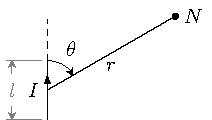
\includegraphics{figAntennaRetardedCurrent}
\caption{برقی رو گزارتی تار کی چھوٹی لمبائی}
\label{شکل_اینٹینا_تاخیری_رو}
\end{figure}

مساوات \حوالہ{مساوات_اینٹینا_تاخیری_رو} کہتا ہے کہ نقطہ \عددیء{N} پر لمحہ \عددیء{t}  پر پیدا اثر،  گزرے  لمحے \عددیء{(t-\tfrac{r}{c})} پر تار میں برقی رو کا اثر ہے جہاں تار سے \عددیء{N} تک فاصلہ \عددیء{r} ہے۔تار سے \عددیء{N} تک شعاع پہنچنے کا دورانیہ \عددیء{\tfrac{r}{c}} ہے۔

گزشتہ بابوں میں امواج کی بات کرتے ہوئے \عددیء{\cos (\omega t -\beta x)} استعمال کیا گیا جس میں \عددیء{\tfrac{\omega}{\beta}=c} کے استعمال سے
\begin{align}
\cos (\omega t -\beta x)=\cos \omega\left( t- \frac{x}{c}\right)
\end{align}
لکھا جا سکتا ہے  جو تاخیری تفاعل کو ظاہر کرتی ہے۔

مساوات \حوالہ{مساوات_اینٹینا_تاخیری_رو} کی دوری سمتیہ شکل
\begin{align}
[I]=I_0 e^{j \omega (t-r/c)}=I_0 e^{j(\omega t-\beta r)}
\end{align}
ہے۔اسی طرح کثافت برقی رو کی تاخیری دوری سمتیہ شکل
\begin{align}
[\kvec{J}]=\kvec{J}_0 e^{j \omega (t-r/c)}=\kvec{J}_0 e^{j(\omega  t -\beta r)}
\end{align}
ہو گی جسے استعمال کرتے ہوئے تاخیری مقناطیسی دباو
\begin{align}\label{مساوات_اینٹینا_تاخیری_سمتی_دباو}
[\kvec{A}]=\frac{\mu}{4\pi}\int_h \frac{[\kvec{J}]}{r}\dif h=\frac{\mu}{4\pi}\int_h \frac{\kvec{J}_0 e^{j\omega(t-r/c)}}{r} \dif h
\end{align}
لکھا جائے گا۔اسی طرح تاخیری حجمی کثافت چارج
\begin{align}
[\rho_h]= \rho_0 e^{j\omega \left(t-r/c \right)}
\end{align}
لکھتے ہوئے تاخیری برقی دباو
\begin{align}\label{مساوات_اینٹینا_تاخیری_مقداری_دباو}
[V]=\frac{1}{4\pi \epsilon}\int_h \frac{[\rho_h]}{ r} \dif h
\end{align}
لکھا جائے گا۔ باب-\حوالہ{باب_میکس_ویل} کے آخر میں مساوات \حوالہ{مساوات_میکس_ویل_تاخیری_سمتی_دباو} اور مساوات \حوالہ{مساوات_میکس_ویل_تاخیری_غیر_سمتی_دباو} کے بائیں ہاتھ کے تفاعل کو چکور قوسین میں لکھ کر موج کی رفتار \عددیء{c} لیتے ہوئے اور فاصلے  کو کروی محدد کے رداس \عددیء{r} سے ظاہر کرنے سے  یہی مساوات حاصل ہوتے ہیں۔


\حصہ{مختصر جفت قطبی اینٹینا}
مختصر لمبائی کے سیدھے موصل تار کو عموماً مختصر \اصطلاح{ جفت قطب}\فرہنگ{جفت قطب!مختصر}\حاشیہب{short dipole}\فرہنگ{dipole!short} کہا جاتا ہے۔مندرجہ ذیل گفتگو میں مختصر جفت قطب کی لمبائی محدود ہو گی۔لامحدود حد تک کم لمبائی کی صورت میں اسے صغاری جفت قطب\فرہنگ{صغاری جفت قطب}\حاشیہب{infinitesimal} کہا جائے گا۔

خطی نوعیت کے کسی بھی اینٹینا کو متعدد تعداد کے سلسلہ وار جڑے مختصر جفت قطبوں کا مجموعہ تصور کیا جا سکتا ہے لہٰذا مختصر جفت قطب کی خاصیت جانتے ہوئے زیادہ لمبے جفت قطب یا مختلف انداز میں جڑے موصل  تاروں کی خاصیت جاننے میں مدد ملے گی۔ 

آئیں شکل \حوالہ{شکل_اینٹینا_جفت_قطب}-الف میں دکھائے مختصر جفت قطب پر غور کریں جس کی لمبائی \عددیء{l} طول موج سے بہت کم \عددیء{l\ll \lambda} ہے۔جفت قطب کے سروں پر موصل چادر بطور  کپیسٹر  بوجھ کردار ادا کرتے ہیں۔جفت قطب کی مختصر لمبائی اور اس کے سروں پر موصل چادر مل کر جفت قطب  کی پوری لمبائی پر تقریباً برابر برقی رو رکھنے میں مدد دیتے ہیں۔جیسے شکل-الف میں دکھایا گیا ہے، جفت قطب کو متوازن ترسیلی تار سے طاقت مہیا کی جا سکتی ہے۔یہ فرض کرتے ہوئے کہ ترسیلی تار سے شعاعی اخراج نہیں ہوتی، اس کے موجودگی کو نظر انداز کیا جائے گا۔جفت قطب کے سروں پر نسب موصل چادروں کے شعاعی اخراج کو بھی نظر انداز کیا جائے گا۔جفت قطب کی موٹائی \عددیء{d} اس کے لمبائی سے بہت کم \عددیء{d\ll \lambda} ہے۔ان حقائق کو مد نظر رکھتے ہوئے تحلیلی تجزیے کی خاطر جفت قطب کو شکل \حوالہ{شکل_اینٹینا_جفت_قطب}-ب کی طرح تصور کیا جا سکتا ہے۔ایسا جفت قطب یکساں برقی رو \عددیء{I} گزارتا، \عددیء{l} لمبائی کا تار معلوم ہو گا جس کے دونوں سروں پر برابر مگر الٹ قطب کے چارج \عددیء{\mp q} ہوں۔کپیسٹر پر چارج \عددیء{q} اور برقی رو \عددیء{I} کا تعلق
\begin{align}\label{مساوات_اینٹینا_رو_اور_چارج}
I=\frac{\partial q}{\partial t}
\end{align}
ہے۔ 

آئیں لامحدود وسعت کی خالی خلاء میں جفت قطب کے میدان حاصل کریں۔جفت قطب کے وسط کو کروی محدد کے مرکز اور لمبائی کو \عددیء{z} محدد پر رکھتے ہوئے آگے بڑھتے ہیں۔کسی بھی نقطہ \عددیء{N} پر عموماً آپس میں عمودی تین میدان \عددیء{E_r}، \عددیء{E_{\theta}} اور \عددیء{E{\phi}} پائے جائیں گے۔

\begin{figure}
\centering
\begin{subfigure}{0.4\textwidth}
\centering
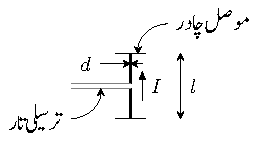
\includegraphics{figAntennaShortDipole}
\caption*{الف: متوازن ترسیلی تار سے جفت قطب کو طاقت مہیا کی گئی ہے۔}
\end{subfigure}%
%
\begin{subfigure}{0.4\textwidth}
\centering
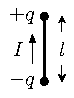
\includegraphics{figAntennaShortDipoleAsShortWire}
\caption*{ب: جفت قطب بطور چھوٹی تار}
\end{subfigure}%
\caption{جفت قطب}
\label{شکل_اینٹینا_جفت_قطب}
\end{figure}


کسی بھی نقطہ \عددیء{N} پر مساوات \حوالہ{مساوات_میکس_ویل_تاخیری_مقناطیسی_میدان}  اور مساوات \حوالہ{مساوات_میکس_ویل_تاخیری_برقی_میدان} بالترتیب مقناطیسی میدان اور برقی میدان دیتے ہیں
\begin{align}
\kvec{H}=\frac{1}{\mu_0}\nabla \times \kvec{A} \\
\kvec{E}=-\nabla V-\frac{\partial \kvec{A}}{\partial t}
\end{align}
جہاں
\begin{description}
\جزو{$V$} نقطہ \عددیء{N} پر مقداری برقی دباو
\جزو{$\kvec{A}$} نقطہ \عددیء{N} پر سمتی دباو
\end{description}
ہیں۔اگر ہمیں کسی بھی نقطے پر مقداری دباو \عددیء{V} اور سمتی دباو \عددیء{\kvec{A}} معلوم ہوں تب مندرجہ بالا دو مساوات سے اس نقطے پر برقی اور مقناطیسی میدان حاصل کئے جا سکتے ہیں۔چونکہ ہمیں  جفت قطب سے دور میدان درکار ہیں لہٰذا ایسی صورت میں مساوات \حوالہ{مساوات_اینٹینا_تاخیری_سمتی_دباو} اور مساوات \حوالہ{مساوات_اینٹینا_تاخیری_مقداری_دباو} میں دئے تاخیری دباو قابل استعمال ہوں گے۔یوں ان مساوات کو
\begin{align}
\kvec{H}&=\frac{1}{\mu_0}\nabla \times [\kvec{A}] \label{مساوات_اینٹینا_عمومی_مقناطیسی}\\
\kvec{E}&=-\nabla [V]-\frac{\partial [\kvec{A}]}{\partial t}=-\nabla [V]-j \omega [\kvec{A}]\label{مساوات_اینٹینا_عمومی_برقی}
\end{align}
لکھا جا سکتا ہے جہاں مساوات \حوالہ{مساوات_میکس_ویل_بدلتا_میدان_غیر_سمتی_دباو} اور مساوات \حوالہ{مساوات_میکس_ویل_بدلتا_میدان_سمتی_دباو} سے تاخیری دباو
\begin{align}
[\kvec{A}]&=\frac{\mu_0}{4\pi} \int_h \frac{\kvec{J}_0 e^{j \omega(t-r/c)}}{r} \dif h \label{مساوات_اینٹینا_عمومی_سمتی_دباو}\\
[V]&=\frac{1}{4\pi\epsilon_0}\int_h \frac{\rho_0 e^{j\omega(t-r/c)}}{r} \dif h\label{مساوات_اینٹینا_عمومی_مقداری_دباو}
\end{align}
لکھے جا سکتے ہیں۔

کسی بھی برقی چارج اور برقی رو سے پیدا میدان مساوات \حوالہ{مساوات_اینٹینا_عمومی_مقناطیسی} اور مساوات \حوالہ{مساوات_اینٹینا_عمومی_برقی} سے حاصل کئے جا سکتے ہیں۔مساوات \حوالہ{مساوات_اینٹینا_عمومی_مقداری_دباو} کے تحت تاخیری مقداری دباو \عددیء{[V]} صرف ساکن چارجوں پر منحصر ہے جبکہ مساوات \حوالہ{مساوات_اینٹینا_عمومی_سمتی_دباو} کے تحت  تاخیری سمتی دباو \عددیء{[\kvec{A}]} صرف برقی رو یعنی حرکت کرتے چارجوں پر منحصر ہے۔مساوات \حوالہ{مساوات_اینٹینا_عمومی_مقناطیسی} کے تحت مقناطیسی میدان \عددیء{\kvec{H}} صرف برقی رو یعنی حرکت کرتے چارجوں پر منحصر ہے جبکہ مساوات \حوالہ{مساوات_اینٹینا_عمومی_برقی} کے تحت برقی میدان \عددیء{\kvec{E}} ساکن چارج اور برقی رو دونوں پر منحصر ہے۔ہم جلد دیکھیں گے کہ کسی بھی چارج اور برقی رو سے  دور پیدا مقناطیسی اور برقی میدانوں کا دارومدار صرف برقی رو پر ہوتا ہے۔ چونکہ اس باب میں تاخیری دباو ہی استعمال کئے جائیں گے لہٰذا انہیں چکور قوسین میں لکھنے سے گریز کیا جائے گا۔اس باب میں یہاں سے آگے بغیر چکور قوسین کے دباو کو تاخیری دباو ہی سمجھا جائے۔

شکل سے ظاہر ہے کہ سمتی دباو کا صرف \عددیء{\az} جزو
\begin{align}\label{مساوات_اینٹینا_جفت_قطب_سمتی_دباو_حصول}
\kvec{A}=\frac{\az \mu_0 }{4\pi} \int_{-l/2}^{l/2} \frac{I_0 e^{j(\omega t -\beta s)}}{s} \dif z
\end{align}
 پایا جاتا ہے۔اگر جفت قطب کی لمبائی \عددیء{l}، نقطہ \عددیء{N} سے جفت قطب تک فاصلہ \عددیء{r} سے نہایت کم \عددیء{l\ll r} اور طول موج \عددیء{\lambda} سے بھی نہایت کم \عددیء{l \ll \lambda} ہو تب مندرجہ بالا مساوات میں متغیر فاصلہ \عددیء{s} کی جگہ مستقل فاصلہ \عددیء{r} پر کیا جا سکتا ہے اور ساتھ ہی ساتھ \عددیء{l} پر مختلف نقطوں سے  \عددیء{N} پر پیدا دباو میں زاویائی فرق کو نظر انداز کیا جا سکتا ہے۔اس طرح ان تمام کو تکمل کے باہر لے جایا جا سکتا ہے۔جفت قطب کی پوری لمبائی پر یک برابر برقی رو \عددیء{I_0} کی صورت میں \عددیء{I_0} کو بھی تکمل کے باہر لے جایا جا سکتا ہے۔یوں مندرجہ بالا مساوات سے
\begin{align}\label{مساوات_اینٹینا_جفت_قطب_سمتی_دباو_حاصل}
\kvec{A} =\frac{\az \mu_0 I_0 l e^{j(\omega t -\beta r)}}{4\pi r}
\end{align}
حاصل ہوتا ہے۔ اس مساوات کو کروی محدد میں یوں
\begin{align*}
\kvec{A}=A_r \ar +A_{\theta} \atheta +A_{\phi} \aphi
\end{align*}
لکھا جائے گا جہاں
\begin{gather}
\begin{aligned}\label{مساوات_اینٹینا_کروی_سمتی_دباو}
A_r&=\ar \cdot \kvec{A}= \frac{ \mu_0 I_0 l e^{j(\omega t -\beta r)}}{4\pi r} \ar \cdot \az= \frac{ \mu_0 I_0 l e^{j(\omega t -\beta r)}}{4\pi r} \cos \theta\\
A_{\theta}&=\atheta \cdot \kvec{A}=\frac{ \mu_0 I_0 l e^{j(\omega t -\beta r)}}{4\pi r} \atheta \cdot \az =-\frac{ \mu_0 I_0 l e^{j(\omega t -\beta r)}}{4\pi r} \sin \theta \\
A_{\phi}&=\aphi \cdot \kvec{A}=\frac{ \mu_0 I_0 l e^{j(\omega t -\beta r)}}{4\pi r} \aphi \cdot \az =0
\end{aligned}
\end{gather}
ہوں گے جہاں اکائی سمتیات کے مقداری ضرب صفحہ \حوالہصفحہ{جدول_سمتیہ_کروی_نلکی_اکائی_غیر-سمتی_ضرب} پر جدول \حوالہ{جدول_سمتیہ_کروی_نلکی_اکائی_غیر-سمتی_ضرب} سے حاصل کئے گئے۔اس طرح 
\begin{align}\label{مساوات_اینٹینا_جفت_قطب_سمتی_دباو}
\kvec{A}=\frac{ \mu_0 I_0 l e^{j(\omega t -\beta r)}}{4\pi r}\left(\cos \theta \ar-\sin \theta \atheta \right)
\end{align}
لکھا جائے گا۔

ساکن چارج جفت قطب کے سروں پر پایا جاتا ہے لہٰذا مقداری دباو
\begin{align}\label{مساوات_اینٹینا_مقداری_دباو_الف}
V=\frac{q_0}{4\pi \epsilon_0} \left[\frac{e^{j(\omega t -\beta s_1)}}{s_1} -\frac{e^{j(\omega t -\beta s_2)}}{s_2}\right]
\end{align}
ہو گا جہاں مساوات \حوالہ{مساوات_اینٹینا_رو_اور_چارج} کے تحت
\begin{align}\label{مساوات_اینٹینا_رو_اور_چارج_ب}
q=\int I \dif t=\frac{I}{j\omega }
\end{align}
کے برابر ہے جہاں
\begin{align*}
I&=I_0 e^{j(\omega t -\beta s)}\\
q&=q_0  e^{j(\omega t -\beta s)}
\end{align*}
ہیں۔مساوات \حوالہ{مساوات_اینٹینا_رو_اور_چارج_ب} سے \عددیء{q_0=\tfrac{I_0}{j\omega}} حاصل کرتے ہوئے مساوات \حوالہ{مساوات_اینٹینا_مقداری_دباو_الف} میں پر کرتے ہیں۔ 
\begin{align}\label{مساوات_اینٹینا_مقداری_دباو_ب}
V=\frac{I_0}{4\pi \epsilon_0 j \omega } \left[\frac{e^{j(\omega t -\beta s_1)}}{s_1} -\frac{e^{j(\omega t -\beta s_2)}}{s_2}\right]
\end{align}
شکل کو دیکھ کر
\begin{align*}
s_1&=r-\frac{l}{2}\cos \theta\\
s_2&=r+\frac{l}{2}\cos \theta
\end{align*}
لکھے جا سکتے ہیں جنہیں مساوات \حوالہ{مساوات_اینٹینا_مقداری_دباو_ب} میں پر کرتے
\begin{align}
V=\frac{I_0 e^{j(\omega t -\beta r)}}{4\pi \epsilon_0 j \omega}\left[\frac{(r+\frac{l}{2}\cos \theta) e^{j\frac{\beta l}{2}\cos \theta}-(r-\frac{l}{2}\cos \theta) e^{-j\frac{\beta l}{2}\cos \theta}}{r^2-\frac{l^2}{4}\cos^2 \theta} \right]
\end{align}
ملتا ہے۔چکور قوسین میں شرح کے نچلے حصے میں \عددیء{r \gg l} کی وجہ سے  \عددیء{\tfrac{l^2}{4}\cos^2 \theta} کو نظر انداز کرتے ہیں۔\اصطلاح{مسئلہ ڈی مویور}\فرہنگ{مسئلہ!ڈی مویور}\فرہنگ{ڈی مویور!مسئلہ}\حاشیہب{$(e^{j\alpha}=\cos \alpha + j \sin \alpha)$ de Moivre's theorem}\فرہنگ{de Moivre} کے استعمال سے
\begin{multline}\label{مساوات_اینٹینا_مقداری_دباو_پ}
V=\frac{I_0 e^{j(\omega t -\beta r)}}{4\pi \epsilon_0 j \omega r^2} \left[\left(r+\frac{l}{2}\cos \theta\right) \left(\cos \frac{\beta l \cos \theta}{2} +j \sin \frac{\beta l \cos \theta}{2}\right)\right.\\
-\left.\left(r-\frac{l}{2}\cos \theta\right) \left(\cos \frac{\beta l \cos \theta}{2} -j \sin \frac{\beta l \cos \theta}{2}\right) \right]
\end{multline}  
لکھا جائے گا۔چونکہ \عددیء{l \ll \lambda} ہے لہٰذا 
\begin{align*}
\cos \frac{\beta l \cos \theta}{2}&=\cos \frac{\pi l \cos \theta}{\lambda}\approx l\\
\sin \frac{\beta l \cos \theta}{2}&\approx \frac{\beta l \cos \theta}{2}
\end{align*}
ہوں گے، جنہیں مساوات \حوالہ{مساوات_اینٹینا_مقداری_دباو_پ} میں پر کرنے سے
\begin{align}\label{مساوات_اینٹینا_مقداری_دباو_ت}
V=\frac{I_0 l e^{j(\omega t -\beta r)} \cos \theta}{4\pi \epsilon_0 c}\left(\frac{1}{r}+\frac{c}{j\omega r^2} \right)
\end{align}
حاصل ہوتا ہے جہاں
\begin{description}
\جزو{$I_0$} برقی رو کا حیطہ یعنی اس کی زیادہ سے زیادہ قیمت، \عددیء{\si{\ampere}}
\جزو{$l$} جفت قطب کی لمبائی، \عددیء{\si{\meter}}
\جزو{$\omega$}  زاویائی تعدد \عددیء{(\omega=2\pi f)} ، اکائی \عددیء{\si{\radian / \second}}۔ جہاں ہرٹز \عددیء{\si{\hertz}}میں تعدد \عددیء{f} ہے
\جزو{$\beta$} زاویائی مستقل \عددیء{(\beta=\tfrac{2\pi}{\lambda})}، اکائی \عددیء{\si{\radian /\meter}}
\جزو{$t$}وقت،\عددیء{\si{\second}} 
\جزو{$\theta$}جفت قطب اور جفت قطب سے نقطہ \عددیء{N} تک سمتیہ کے مابین زاویہ
\جزو{$\epsilon_0$}خالی خلاء کا برقی مستقل، \عددیء{\SI{8.854}{\pico\farad/\meter}}
\جزو{$c$}خالی خلاء میں شعاع کی رفتار، \عددیء{\SI{3e8}{\meter/\second}}
\جزو{$j$}خیالی عدد \عددیء{\sqrt{-1}}
\جزو{$r$}جفت قطب کے وسط سے نقطہ \عددیء{N} تک فاصلہ،\عددیء{\si{\meter}}
\end{description}
ہیں۔

مختصر جفت قطب کے وسط سے، \عددیء{l \ll \lambda} اور \عددیء{l \ll r} کی صورت میں، \عددیء{r} فاصلے اور \عددیء{\theta} زاویے پر مساوات \حوالہ{مساوات_اینٹینا_جفت_قطب_سمتی_دباو} سمتی دباو اور مساوات \حوالہ{مساوات_اینٹینا_مقداری_دباو_ت} مقداری دباو دیتے ہیں۔کروی محدد میں مقداری دباو کی ڈھلوان
\begin{gather}
\begin{aligned}
\nabla V&=\frac{\partial V}{\partial r}\ar+\frac{1}{r}\frac{\partial V}{\partial \theta}\atheta+\frac{1}{r\sin \theta} \frac{\partial V}{\partial \phi}\aphi\\
&=\frac{I_0 l e^{j(\omega t -\beta r)}}{4\pi \epsilon_0 c}\left[-\left(\frac{ \cos \theta}{r^2}+\frac{2 c  \cos \theta}{j\omega r^3} \right)\ar -\left(\frac{\sin \theta}{r}+\frac{c \sin \theta}{j\omega r^2} \right) \atheta\right]
\end{aligned}
\end{gather}
کے برابر ہے۔برقی میدان \عددیء{\kvec{E}=E_r \ar +E_{\theta} \atheta+E_{\phi}\aphi} کے اجزاء مساوات \حوالہ{مساوات_اینٹینا_عمومی_برقی} کی مدد سے 
\begin{align*}
E_r&=-\frac{\partial V}{\partial r}-j \omega A_r\\
E_{\theta}&=-\frac{1}{r}\frac{\partial V}{\partial \theta}-j \omega A_{\theta}\\
E_{\phi}&=-\frac{1}{r\sin \theta}\frac{\partial V}{\partial \phi}-j \omega A_{\phi}
\end{align*}
لکھے جا سکتے ہیں جن میں مطلوبہ تفاعل پر کرنے سے برقی میدان کے عمومی مساوات
\begin{gather}
\begin{aligned}\label{مساوات_اینٹینا_جفت_قطب_برقی_اجزاء}
E_r&=\frac{I_0 l \cos \theta e^{j(\omega t -\beta r)}}{2\pi \epsilon_0}\left(\frac{1}{c r^2}+\frac{1}{j \omega r^3} \right)\\
E_{\theta}&=\frac{I_0 l \sin \theta e^{j(\omega t -\beta r)}}{4\pi \epsilon_0}\left(\frac{j \omega}{c^2 r}+\frac{1}{c r^2}+\frac{1}{j \omega r^3} \right)\quad \quad \text{\RL{عمومی میدان}}\\
E_{\phi}&=0 
\end{aligned}
\end{gather}
حاصل ہوتے ہیں۔

مقناطیسی میدان مساوات \حوالہ{مساوات_اینٹینا_عمومی_مقناطیسی} سے حاصل ہو گی۔کروی محدد میں سمتی دباو کی گردش
\begin{multline}
\kvec{B}=\nabla \times \kvec{A}=\frac{1}{r \sin \theta}\left[\frac{\partial (A_{\theta}  \sin \theta)}{\partial \theta}-\frac{\partial A_{\theta} }{\partial \phi} \right]\ar+\frac{1}{r }\left[\frac{1}{\sin \theta}\frac{\partial A_r }{\partial \phi}-\frac{\partial (r A_{\phi} )}{\partial r} \right]\atheta
\\
 +\frac{1}{r}\left[\frac{\partial (r A_\theta )}{\partial r}-\frac{\partial A_r }{\partial \theta} \right]\aphi
\end{multline}
میں مساوات \حوالہ{مساوات_اینٹینا_کروی_سمتی_دباو} پر کرنے سے مقناطیسی میدان کی عمومی مساوات
\begin{gather}
\begin{aligned}\label{مساوات_اینٹینا_جفت_قطب_مقناطیسی_اجزاء}
H_{\phi}&=\frac{I_0 l \sin \theta e^{j(\omega t -\beta r)}}{4\pi} \left(\frac{j \omega}{c r}+\frac{1}{r^2} \right)\quad \quad\text{\RL{عمومی میدان}}\\
H_r&=0\\
H_{\theta}&=0 
\end{aligned}
\end{gather}
حاصل ہوتے ہیں جہاں \عددیء{\kvec{B}=\mu_0 \kvec{H}} کا استعمال کیا گیا۔

مساوات \حوالہ{مساوات_اینٹینا_جفت_قطب_برقی_اجزاء} اور مساوات \حوالہ{مساوات_اینٹینا_جفت_قطب_مقناطیسی_اجزاء} کے تحت جفت قطب سے پیدا  میدان کے صرف تین اجزاء \عددیء{E_r}، \عددیء{E_{\theta}} اور \عددیء{H_{\phi}} پائے جاتے ہیں۔جفت قطب سے زیادہ فاصلے پر میدان کی مساوات میں \عددیء{\tfrac{1}{r^2}} یا \عددیء{\tfrac{1}{r^3}} کو نظر انداز کیا جا سکتا ہے۔یوں \عددیء{E_r} قابل نظر انداز ہو گا لہٰذا \عددیء{E_r \approx 0} تصور کیا جائے گا جبکہ
\begin{gather}
\begin{aligned}\label{مساوات_اینٹینا_جفت_قطب_دور_میدان}
E_{\theta}&=\frac{I_0 l \sin \theta e^{j(\omega t -\beta r)}}{4\pi \epsilon_0 }\frac{j \omega}{c^2 r}=j \frac{30 I_0 \beta l}{r} \sin \theta e^{j(\omega t-\beta r)}\\
H_{\phi}&=\frac{ I_0 l \sin \theta e^{j(\omega t -\beta r)}}{4\pi }\frac{j \omega}{c r}=j\frac{I_0 \beta l}{4\pi r} \sin \theta e^{j(\omega t -\beta r)}\quad \quad \text{\RL{دور میدان}}
\end{aligned}
\end{gather} 
ہوں گے۔مساوات \حوالہ{مساوات_اینٹینا_جفت_قطب_دور_میدان} استعمال کرتے ہوئے برقی اور مقناطیسی میدان کی شرح
\begin{align}
\frac{E_{\theta}}{H_{\phi}}=\frac{1}{\epsilon_0 c}=\sqrt{\frac{\mu_0}{\epsilon_0}}=\SI{376.7}{\ohm}
\end{align}
حاصل ہوتی ہے جو خالی خلاء کی قدرتی رکاوٹ ہے۔

یہاں اس حقیقت پر توجہ دیں کہ خالی خلاء میں \عددیء{\TEM} موج کی طرح، جفت قطب سے دور \عددیء{E_{\theta}} اور \عددیء{H_{\phi}}  آپس میں ہم قدم ہیں۔اس کے علاوہ دونوں میدان  \عددیء{\sin \theta} کے راست تناسب ہیں یعنی جفت قطب کے محوری سمت \عددیء{\theta=0^{\circ}} پر ان کی قیمت صفر جبکہ \عددیء{\theta=90^{\circ}} پر ان کی قیمت زیادہ سے زیادہ ہے۔اندرسہ\فرہنگ{اندرسہ}\حاشیہب{doughnut}\فرہنگ{doughnut} شکل کی ان میدان کو شکل میں دکھایا گیا ہے۔

جفت قطب سے دور میدان حاصل کرتے وقت مساوات \حوالہ{مساوات_اینٹینا_جفت_قطب_برقی_اجزاء} اور مساوات \حوالہ{مساوات_اینٹینا_جفت_قطب_مقناطیسی_اجزاء} میں \عددیء{\tfrac{1}{r^2}} یا \عددیء{\tfrac{1}{r^3}} رکھتے اجزاء کو نظر انداز کیا گیا یعنی \عددیء{E_{\theta}} میں 
\begin{align*}
\abs{j\frac{ \omega}{c^2 r}} & \gg \frac{1}{c r^2}\\
\abs{j\frac{ \omega}{c^2 r}} &\gg \abs{\frac{1}{j \omega r^3}} 
\end{align*}
یا
\begin{align}
r \gg \frac{c}{\omega}
\end{align}
تصور کیا گیا۔اسی طرح \عددیء{H_{\phi}} میں بھی
\begin{align*}
\abs{j \frac{ \omega}{c r}} \gg \frac{1}{r^2}
\end{align*}
یا
\begin{align}
r \gg \frac{c}{\omega}
\end{align}
تصور کیا گیا جسے
\begin{align}
r \gg \frac{1}{\beta} \quad \quad (\text{\RL{دور میدان}})
\end{align}
بھی لکھا جا سکتا ہے۔اگر جفت قطب کے قریب میدان کی بات کی جائے تو \عددیء{r \ll \tfrac{c}{\omega}} یعنی \عددیء{r \ll \tfrac{1}{\beta}} لیا جائے گا۔یوں مساوات \حوالہ{مساوات_اینٹینا_جفت_قطب_برقی_اجزاء} اور مساوات \حوالہ{مساوات_اینٹینا_جفت_قطب_مقناطیسی_اجزاء} میں
\begin{align*}
\frac{1}{c r^2}& \ll \abs{\frac{1}{j \omega r^3}}\\
\abs{\frac{j \omega}{c^2 r}}& \ll \abs{\frac{1}{j \omega r^3}}\\
\frac{1}{c r^2}& \ll \abs{\frac{1}{j \omega r^3}} \\
\abs{\frac{j \omega}{c r}}& \ll \frac{1}{r^2}
\end{align*}
ہوں گے لہٰذا قریبی میدان
\begin{gather}
\begin{aligned}\label{مساوات_اینٹینا_جفت_قطب_قریب_میدان}
E_r&=\frac{I_0 l \cos \theta e^{j(\omega t -\beta r)}}{2\pi \epsilon_0 }\frac{1}{j \omega r^3} =\frac{I_0 l \cos \theta e^{j(\omega t -\beta r-\tfrac{\pi}{2})}}{2\pi \epsilon_0 \omega r^3}\\
E_{\theta}&=\frac{I_0 l \sin \theta e^{j(\omega t -\beta r)}}{4\pi \epsilon_0}\frac{1}{j \omega r^3}=\frac{I_0 l \sin \theta e^{j(\omega t -\beta r-\tfrac{\pi}{2})}}{4\pi \epsilon_0 \omega r^3}\\
H_{\phi}&=\frac{I_0 l \sin \theta e^{j(\omega t -\beta r)}}{4\pi}\frac{1}{r^2}=\frac{I_0 l \sin \theta e^{j(\omega t -\beta r)}}{4\pi r^2} \quad \text{\RL{قریبی میدان}}
\end{aligned}
\end{gather}
لکھے جا سکتے ہیں۔ کل قریبی برقی میدان
\begin{align}\label{مساوات_اینٹینا_قریب_کل_برقی}
\kvec{E}=E_r \ar+E_{\theta}\atheta=\left[\frac{I_0 l \cos \theta }{2\pi \epsilon_0 \omega r^3}\ar+\frac{I_0 l \sin \theta }{4\pi \epsilon_0 \omega r^3}\atheta\right]e^{j(\omega t -\beta r-\tfrac{\pi}{2})}
\end{align}
ہو گا۔مساوات \حوالہ{مساوات_اینٹینا_قریب_کل_برقی} کے برقی میدان میں جزو ضربی \عددیء{e^{j(\omega t -\beta r-\tfrac{\pi}{2})}} پایا جاتا ہے جبکہ مقناطیسی میدان میں جزو ضربی \عددیء{e^{j(\omega t -\beta r)}} پایا جاتا ہے۔یوں جفت قطب کے قریب کسی بھی نقطے پر ہر لمحہ برقی میدان  اور مقناطیسی میدان میں \عددیء{\tfrac{\pi}{2}} زاویے کا فرق پایا جاتا ہے جو ساکن میدان کی نشانی ہے۔

جفت قطب کے قریب برقی اور مقناطیسی میدان میں لمحاتی طور \عددیء{\tfrac{\pi}{2}} ریڈیئن  کا زاویہ پایا جاتا ہے جبکہ جفت قطب سے دور دونوں میدان لمحاتی طور پر ہم قدم ہیں لہٰذا کسی درمیانے فاصلے پر ان میدانوں میں \عددیء{45^{\circ}} کا زاویہ ہو گا۔آپ دیکھ سکتے ہیں کہ جفت قطب سے فاصلہ بڑھانے سے برقی میدان وقت کی نسبت سے گھوم کر مقناطیسی میدان کے ہم قدم ہو جاتا ہے۔

مخلوط پوئنٹنگ سمتیہ استعمال کرتے ہوئے مساوات \حوالہ{مساوات_اینٹینا_جفت_قطب_دور_میدان} سے  دور میدان میں کثافت توانائی
\begin{align*}
\pmb{\mathscr{P}}_{\text{اوسط}}=\frac{1}{2}\left[\kvec{E} \times \kvec{H}^*\right]_{\text{حقیقی}}=\frac{1}{2}E_{\theta} H_{\phi}^* \ar=\frac{15 I_0^2 \beta^2 l^2}{4 \pi r^2} \sin^2 \theta \ar \quad \text{\RL{دور کثافت طاقت}}
\end{align*}
حاصل ہوتی ہے جو  رداسی \عددیء{r} سمت میں منتقل ہوتی حقیقی توانائی ہے۔یہی اینٹینا کی شعاعی اخراج ہے۔شعاعی اخراج \عددیء{\theta=90^{\circ}} پر زیادہ سے زیادہ ہے۔اسی طرح پوئنٹنگ سمتیہ استعمال کرتے ہوئے مساوات \حوالہ{مساوات_اینٹینا_جفت_قطب_قریب_میدان} سے قریبی میدان میں کثافت توانائی
\begin{align*}
\frac{1}{2}\left[\kvec{E} \times \kvec{H}^*\right]_{\text{حقیقی}}&=\frac{1}{2}\left[(E_{r} \ar+E_{\theta} \atheta) \times H_{\phi}^* \aphi\right]_{\text{حقیقی}}\\
&=\frac{1}{2}\left[-\frac{I_0 l \cos \theta }{2\pi \epsilon_0 \omega r^3}\atheta+\frac{I_0 l \sin \theta }{4\pi \epsilon_0 \omega r^3}\ar \right]\frac{I_0 l \sin \theta }{4\pi r^2} e^{-j\tfrac{\pi}{2}}\\
\end{align*}
حاصل ہوتی ہے جس کا بیشتر حصہ خیالی ہے اور ساتھ ہی ساتھ شعاعی اخراج کے علاوہ یہاں \عددیء{\theta} سمت میں گھومتی طاقت بھی پائی جاتی ہے۔

آئیں اب نہایت کم تعدد پر صورت حال دیکھیں۔ مساوات \حوالہ{مساوات_اینٹینا_جفت_قطب_برقی_اجزاء} میں \عددیء{I_0=j \omega q_0} پر کرتے ہوئے اور مساوات \حوالہ{مساوات_اینٹینا_جفت_قطب_مقناطیسی_اجزاء} کو جوں کا توں دوبارہ پیش کرتے ہیں۔
\begin{align*}
E_r&=\frac{q_0 l \cos \theta e^{j(\omega t -\beta r)}}{2\pi \epsilon_0}\left(\frac{j \omega}{c r^2}+\frac{1}{ r^3} \right)\\
E_{\theta}&=\frac{q_0 l \sin \theta e^{j(\omega t -\beta r)}}{4\pi \epsilon_0}\left(-\frac{\omega^2 }{c^2 r}+\frac{j \omega }{c r^2}+\frac{1}{ r^3} \right)\\
H_{\phi}&=\frac{I_0 l \sin \theta e^{j(\omega t -\beta r)}}{4\pi} \left(\frac{j \omega}{c r}+\frac{1}{r^2} \right)
\end{align*}
\عددیء{\abs{e^{-j\beta r}}=1} لیتے ہوئے، صفر کے قریب تر تعدد \عددیء{\omega \to 0} پر ان مساوات سے میدان کی حتمی قیمت
\begin{align*}
E_r&=\frac{q_0 l \cos \theta}{2\pi \epsilon_0 r^3}\\
E_{\theta}&=\frac{q_0 l \sin \theta }{4\pi \epsilon_0 r^3}\\
H_{\phi}&=\frac{I_0 l \sin \theta }{4\pi r^2} \quad \quad \text{\RL{نیم ساکن میدان}}
\end{align*}
حاصل ہوتی ہیں جن سے برقی میدان
\begin{align}
\kvec{E}=\frac{q_0 l }{4\pi \epsilon_0 r^3}\left(2\cos \theta \ar+\sin \theta \atheta \right)
\end{align}
لکھا جا سکتا ہے۔ان میدان کو \اصطلاح{نیم ساکن میدان}\فرہنگ{میدان!نیم ساکن}\حاشیہب{quasi stationary fields}\فرہنگ{quasi stationary fields} کہا جاتا ہے۔یہ صفحہ \حوالہصفحہ{مساوات_توانائی_جفت_قطب_دور_میدان_الف} پر حاصل کی گئی مساوات \حوالہ{مساوات_توانائی_جفت_قطب_دور_میدان_الف} ہی ہے۔اسی طرح مندرجہ بالا مقناطیسی میدان \عددیء{H_{\phi}} کی قیمت صفحہ \حوالہصفحہ{مساوات_مقناطیسی_تار_کا_ٹکڑا_اور_میدان} پر مساوات \حوالہ{مساوات_مقناطیسی_تار_کا_ٹکڑا_اور_میدان} ہی ہے۔چونکہ یہ میدان \عددیء{\tfrac{1}{r^2}} یا \عددیء{\tfrac{1}{r^3}} کے تعلق سے تبدیل ہوتے ہیں لہٰذا یہ جفت قطب کے قریب ہی پائے جاتے ہیں۔جفت قطب سے دور ان کی قیمت قابل نظر انداز ہوتی ہے لہٰذا ان کا شعاعی اخراج میں خاص کردار نہیں ہوتا۔بلند تعدد پر دور میدان جنہیں مساوات \حوالہ{مساوات_اینٹینا_جفت_قطب_دور_میدان} پیش کرتی ہے، \عددیء{\tfrac{1}{r}} کے تعلق سے گھٹتی ہیں لہٰذا یہی شعاعی اخراج کو ظاہر کرتی ہیں اور یوں انہیں \اصطلاح{اخراجی میدان}\فرہنگ{اخراجی میدان}\حاشیہب{radiation fields}\فرہنگ{radiation fields} کہا جاتا ہے۔

مختصر جفت قطب، \عددیء{l \ll r} اور \عددیء{l \ll \lambda}، کے تمام میدان کو جدول \حوالہ{جدول_اینٹینا_مختصر_جفت_قطب} میں پیش کیا گیا ہے۔بقایا اجزاء \عددیء{E_{\phi}=H_r=H_{\theta}=0} صفر  کے برابر ہیں۔
\begin{table}
\caption{مختصر جفت قطب کے میدان}
\centering
\begin{tabular}{l l l l}
\hline
جزو & عمومی مساوات & دور میدان & نیم ساکن میدان\\
\hline 
\rule{0pt}{2em}
$E_r$ &$\frac{I_0 l \cos \theta e^{j(\omega t -\beta r)}}{2\pi \epsilon_0}\left(\frac{1}{c r^2}+\frac{1}{j \omega r^3} \right)$&$0$&$\frac{q_0 l \cos \theta}{2\pi \epsilon_0 r^3}$ \\[4ex]
$E_{\theta}$&$\frac{I_0 l \sin \theta e^{j(\omega t -\beta r)}}{4\pi \epsilon_0}\left(\frac{j \omega}{c^2 r}+\frac{1}{c r^2}+\frac{1}{j \omega r^3} \right)$&$ \frac{j 60 \pi I_0 \sin \theta e^{j(\omega t-\beta r)}}{r} \frac{l}{\lambda}$& $\frac{q_0 l \sin \theta }{4\pi \epsilon_0 r^3}$\\ [4ex]
$H_{\phi}$&$\frac{I_0 l \sin \theta e^{j(\omega t -\beta r)}}{4\pi} \left(\frac{j \omega}{c r}+\frac{1}{r^2} \right)$&$\frac{j I_0 \sin \theta e^{j(\omega t -\beta r)}}{2r}\frac{l}{\lambda}  $& $\frac{I_0 l \sin \theta }{4\pi r^2} $
\end{tabular}
\label{جدول_اینٹینا_مختصر_جفت_قطب}
\end{table}

اگر ہماری دلچسپی صرف دور میدان میں ہو تب مطلوبہ میدان کو نہایت آسانی کے ساتھ صرف \عددیء{\kvec{A}} سے حاصل کیا جا سکتا ہے چونکہ دور میدان میں مقداری دباو \عددیء{V} کا کوئی کردار نہیں۔یوں مساوات \حوالہ{مساوات_اینٹینا_عمومی_برقی} اور مساوات \حوالہ{مساوات_اینٹینا_کروی_سمتی_دباو} سے
\begin{align}
E_{\theta}&=-j \omega A_{\theta}=-j \omega \left(-\frac{ \mu_0 I_0 l e^{j(\omega t -\beta r)}}{4\pi r} \sin \theta \right)=j \frac{30 I_0 \beta l}{r} \sin \theta e^{j(\omega t-\beta r)}
\end{align}
حاصل ہوتا ہے۔مقناطیسی میدان \عددیء{H_\phi} کو مساوات \حوالہ{مساوات_اینٹینا_عمومی_مقناطیسی} سے حاصل کیا جا سکتا ہے  جہاں \عددیء{\tfrac{1}{r^2}} اجزاء رد کئے جائیں گے۔مقناطیسی میدان  کو نسبتاً زیادہ آسانی سے، لامحدود خلاء کی قدرتی
 رکاوٹ \عددیء{Z_0=\sqrt{\tfrac{\mu_0}{\epsilon_0}}=120\pi} استعمال کرتے ہوئے
\begin{align}
H_{\phi}=\frac{E_{\theta}}{Z_0}=j \frac{30 I_0 \beta l}{120 \pi r} \sin \theta e^{j(\omega t-\beta r)}=j \frac{ I_0 \beta l}{4 \pi r} \sin \theta e^{j(\omega t-\beta r)}
\end{align}
سے بھی  حاصل کیا جا سکتا ہے۔

مساوات \حوالہ{مساوات_اینٹینا_جفت_قطب_دور_میدان} میں \عددیء{\beta=\tfrac{2\pi}{\lambda}} پر کرتے ہوئے دور برقی میدان کو
\begin{align}
E_{\theta}=&j \quad 60 \pi  \quad  I_0  \quad  \frac{l}{\lambda} \quad \frac{1}{r} \quad \sin \theta \quad e^{j(\omega t-\beta r)}\\
&\phantom{j} \quad \underset{\text{مقدار}}{\phantom{60 \pi}}  \quad  \underset{\text{رو}}{\phantom{I_0}}  \enskip  \underset{\text{لمبائی}}{\phantom{l}} \quad  \underset{\text{فاصلہ}}{\phantom{r}} \quad  \underset{\text{شکل}}{\phantom{\sin }} \quad  \underset{\text{زاویہ}}{\phantom{e^{j(\omega t-\beta r)}}} \nonumber
\end{align}
لکھا جا سکتا ہے جہاں \عددیء{60 \pi} جزو مقدار ہے، \عددیء{I_0} برقی رو، \عددیء{\tfrac{l}{\lambda}} جفت قطب کی لمبائی جسے طول موج میں ناپا گیا ہے، \عددیء{\tfrac{1}{r}} فاصلے کو ظاہر کرتا ہے، \عددیء{\sin \theta} میدان کی شکل اور \عددیء{e^{j(\omega t -\beta r)}} زاویائی فرق ہے۔کسی بھی اینٹینا کے میدان کو عموماً ان چھ اجزاء کے حاصل ضرب کی صورت میں لکھا جا سکتا ہے۔

جدول \حوالہ{جدول_اینٹینا_مختصر_جفت_قطب} مختصر جفت قطب کے میدان دیتا ہے۔کسی بھی اینٹینا کو متعدد مختصر جفت قطب کا مجموعہ تصور کیا جا سکتا ہے۔یوں کسی بھی اینٹینا کے میدان تمام جفت قطب کے میدان کو جمع کرتے ہوئے حاصل کیا جا سکتا ہے۔ 

\حصہ{مختصر جفت قطب کا اخراجی مزاحمت}
اینٹینا کے گرد کسی بھی بند سطح پر مخلوط پوئنٹنگ سمتیہ
\begin{align}
\pmb{\mathscr{P}}_{\text{اوسط}}=\frac{1}{2}\left[\kvec{E}_s \times \kvec{H}_s^* \right]_{\text{حقیقی}}
\end{align}
  کی سطحی تکمل
\begin{align}
P=\int_S \pmb{\mathscr{P}}_{\text{اوسط}} \cdot \dif \kvec{s} \quad \quad (\si{\watt})
\end{align}
 کل شعاعی اخراج \عددیء{P} دے گی۔فی سیکنڈ خارج ہونے والی توانائی شعاعی اخراج کہلاتی ہے لہٰذا اس کی اکائی واٹ \عددیء{\si{\watt}} ہے۔سادہ ترین بند سطح کرہ ہے۔یوں اینٹینا کو کروی محدد کے مرکز پر رکھتے ہوئے تکمل حاصل کیا جائے گا۔چونکہ دور کے میدان نسبتاً سادہ صورت رکھتے ہیں لہٰذا بند سطح کا رداس جتنا زیادہ رکھا جائے تکمل اتنا آسان ہو گا۔یوں رداس زیادہ سے زیادہ رکھتے ہوئے دور میدان استعمال کرتے ہوئے جفت قطب کا شعاعی اخراج \عددیء{P} حاصل کیا جاتا ہے۔

کامل اینٹینا کی صورت میں شعاعی اخراج اس برقی طاقت کے برابر ہو گا جو اینٹینا کے برقی سروں پر مہیا کی گئی ہو۔اینٹینا کو مزاحمت \عددیء{R} تصور کرتے ہوئے اس برقی طاقت کو \عددیء{P=\frac{1}{2}I_0^2 R} لکھا جا سکتا ہے جہاں \عددیء{I_0} سائن نما برقی رو کا حیطہ ہے۔یوں
\begin{align}\label{مساوات_اینٹینا_اخراجی_مزاحمت}
R=\frac{2P}{I_0^2} \quad \quad (\si{\ohm})
\end{align}
لکھا جا سکتا ہے جہاں \عددیء{R} اینٹینا کی \اصطلاح{اخراجی مزاحمت}\فرہنگ{اخراج!مزاحمت}\فرہنگ{مزاحمت!اخراجی}\حاشیہب{radiation resistance}\فرہنگ{radiation!resistance}\فرہنگ{resistance!radiation} کہلاتی ہے۔

آئیں مختصر جفت قطب کی اخراجی مزاحمت حاصل کریں۔دور میدان میں صرف \عددیء{E_\theta} اور \عددیء{H_\phi} پائے جاتے ہیں لہٰذا شعاعی اخراج
\begin{align}
P=\frac{1}{2}\int_S \left[E_{\theta} H_{\phi}^{*}\right]_{\text{حقیقی}} \dif s
\end{align} 
سے حاصل ہو گی جہاں \عددیء{H_\phi^*} مقناطیسی میدان \عددیء{H_\phi} کا جوڑی دار مخلوط ہے۔اب \عددیء{E_{\theta}=Z_0 H_{\phi}} ہے لہٰذا
 \begin{align}\label{مساوات_اینٹینا_جفت_قطب_اخراج}
P=\frac{1}{2}\int_S \left[ H_{\phi}H_{\phi}^{*} Z_0\right]_{\text{حقیقی}} \dif s=\frac{Z_0}{2}\int_S  \abs{H_{\phi}}^2  \dif s
\end{align} 
یا
 \begin{align}\label{مساوات_اینٹینا_جفت_قطب_اخراج_ب}
P=\frac{1}{2 Z_0}\int_S  \abs{E_{\phi}}^2  \dif s
\end{align} 
لکھا جا سکتا ہے جہاں خالی خلاء کی قدرتی رکاوٹ  \عددیء{Z_0=\sqrt{\frac{\mu_0}{\epsilon_0}}=120\pi} اور \عددیء{\dif s=r^2 \sin \theta \dif \theta \dif \phi} کے برابر ہیں۔

جفت قطب کے میدان حاصل کرتے وقت فرض کیا گیا کہ اس کی پوری لمبائی پر یک برابر برقی رو \عددیء{I_0} پائی جاتی ہے۔ساتھ ہی ساتھ لمبائی \عددیء{l} کے مختلف نقطوں کے میدان کا زاویائی فرق نظر انداز کیا گیا۔جفت قطب کی پوری لمبائی پر برابر برقی رو نہ ہونے  کی صورت میں مساوات \حوالہ{مساوات_اینٹینا_جفت_قطب_سمتی_دباو_حصول} سے مساوات \حوالہ{مساوات_اینٹینا_جفت_قطب_سمتی_دباو_حاصل} حاصل ہونے کی بجائے
\begin{align*}
\kvec{A} &=\frac{\az \mu_0  e^{j(\omega t -\beta r)}}{4\pi r}\int_{-l/2}^{l/2} i \dif z \\
&=\frac{\az \mu_0 l I e^{j(\omega t -\beta r)}}{4\pi r}
\end{align*}
حاصل ہو گا جہاں \عددیء{I} اوسط برقی رو ہے۔اسی حقیقت کو مد نظر رکھتے ہوئے مساوات \حوالہ{مساوات_اینٹینا_جفت_قطب_دور_میدان} سے مقناطیسی میدان کا حیطہ
\begin{align}
H_{\phi}=\frac{I \beta l}{4\pi r} \sin \theta 
\end{align}
لکھتے ہوئے \عددیء{I_0} کی جگہ اوسط برقی رو \عددیء{I} لکھی گئی ہے۔مقناطیسی میدان کے اس حیطے  کو مساوات \حوالہ{مساوات_اینٹینا_جفت_قطب_اخراج} میں پر کرتے ہوئے زیادہ سے زیادہ اخراجی طاقت 
 \begin{align*}
P&=\frac{120\pi}{2 }\int_0^{2\pi}\int_0^{\pi} \left(\frac{I \beta l}{4\pi r} \sin \theta \right)^2  r^2 \sin \theta \dif \theta \dif \phi\\
&=\frac{120\pi}{2 }\left(\frac{\beta I l}{4\pi}\right)^2\int_0^{2\pi}\int_0^{\pi}  \sin^3 \theta \dif \theta \dif \phi\\
&=80 \pi^2 I^2\left(\frac{l}{\lambda}\right)^2
\end{align*} 
حاصل ہوتی ہے۔مساوات \حوالہ{مساوات_اینٹینا_جفت_قطب_اخراج} یا مساوات \حوالہ{مساوات_اینٹینا_جفت_قطب_اخراج_ب} برقی رو کی چوٹی \عددیء{I} کی صورت میں اخراجی  طاقت دیتے ہیں جو سائن نما برقی رو کی صورت میں اوسط اخراجی طاقت کے دگنا ہوتی ہے۔یوں اوسط اخراجی طاقت
\begin{align}
P_{\text{اوسط}}  &= 40 \pi^2 I^2\left(\frac{l}{\lambda}\right)^2
\end{align} 
ہو گی۔مساوات \حوالہ{مساوات_اینٹینا_اخراجی_مزاحمت} سے مختصر جفت قطب کی اخراجی مزاحمت 
\begin{align}\label{مساوات_اینٹینا_اخراجی_مزاحمت_جفت_قطب}
R=80 \pi^2 \left(\frac{l}{\lambda}\right)^2  \left(\frac{I}{I_0} \right)^2\quad \quad (\si{\ohm})
\end{align}
حاصل ہوتی ہے۔

کسی بھی اینٹینا کی اخراجی مزاحمت
\begin{align}
R=\frac{Z_0}{I_0^2} \int_S \abs{H}^2 \dif s=\frac{1}{Z_0 I_0^2} \int_S \abs{E}^2 \dif s
\end{align}
سے حاصل کی جا سکتی ہے جہاں \عددیء{Z_0=120\pi} کے برابر ہے۔
%============================
\ابتدا{مثال}\شناخت{مثال_اینٹینا_کھمبا_اینٹینا}
چالیس میٹر لمبے کھمبے اینٹینا کو موصل سطح پر کھڑا کئے  \عددیء{\SI{300}{\kilo \hertz}} کے تعدد پر استعمال کیا جاتا ہے۔اسے برقی اشارہ نچلے سرے پر فراہم کیا جاتا ہے۔اینٹینا کی اخراجی مزاحمت حاصل کریں۔اس کھمبے کو شکل \حوالہ{شکل_اینٹینا_کھمبا} میں دکھایا گیا ہے۔کھمبے کو غیر موصل بنیاد پر کھڑا کیا گیا ہے۔

\begin{figure}
\centering
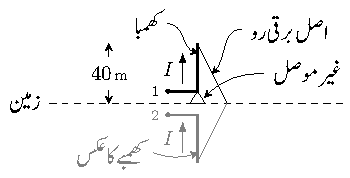
\includegraphics{figAntennaMastAndItsImage}
\caption{کھمبا اینٹینا}
\label{شکل_اینٹینا_کھمبا}
\end{figure}
حل:موصل زمین میں کھمبا اینٹینا کا عکس بنتا ہے۔درکار تعدد پر \عددیء{\lambda=\tfrac{c}{f}=\tfrac{3\times 10^{8}}{300000}=\SI{1000}{\meter}} ہے جو کھمبے کی لمبائی سے بہت زیادہ ہے۔یوں اینٹینا اور اس کا عکس بطور مختصر جفت قطب کردار ادا کرتے ہیں۔چونکہ کھمبے کے سر پر موصل چادر نسب نہیں کیا گیا ہے لہٰذا اس کے پورے لمبائی پر برابر برقی رو تصور کرنا غلط ہو گا۔حقیقت میں، جیسے شکل میں وضاحت کی گئی ہے، کھمبے کے کھلے سر پر برقی رو صفر ہو گی جبکہ نچلے سر پر اس کی قیمت زیادہ سے زیادہ ہو گی۔جیسا شکل میں دکھایا گیا ہے، برقی رو بالمقابل لمبائی \عددیء{l}  کا خط تکونی ہے۔یوں اوسطاً برقی رو \عددیء{I_{\text{اوسط}}=\tfrac{I_0}{2}} ہو گی جہاں برقی رو کی زیادہ سے زیادہ قیمت \عددیء{I_0} ہے۔

یوں \عددیء{2\times 40} میٹر  لمبے فرضی جفت قطب کی اخراجی مزاحمت مساوات \حوالہ{مساوات_اینٹینا_اخراجی_مزاحمت_جفت_قطب} سے 
\begin{align*}
80 \pi^2 \left(\frac{2 \times 40}{1000}\right)^2  \left(\frac{0.5 I_0}{I_0} \right)^2=\SI{1.2633}{\ohm}
\end{align*} 
حاصل ہوتی ہے۔یہ مزاحمت حقیقی کھمبے کے سر \عددیء{1} اور عکسی کھمبے کے سر \عددیء{2} کے مابین ہے۔یوں اصل اینٹینا کی اخراجی مزاحمت جو زمین اور \عددیء{1} کے مابین ناپی جائے گی کی قیمت
\begin{align}
R_{\text{اخراجی}}=\frac{0.63165}{2}=\SI{0.63}{\ohm}
\end{align}
ہو گی۔
\انتہا{مثال}
%==============


حقیقی دھات کامل موصل نہیں ہوتے لہٰذا کسی بھی دھات سے بنائے گئے جفت قطب میں توانائی کا ضیاع ہو گا۔موصل کے علاوہ اینٹینا کے ساتھ منسلک ذو برق میں بھی طاقت کا ضیاع ہو گا۔ان ضیاع کو مزاحمت \عددیء{R_{\text{ضیاعی}}} سے ظاہر کیا جا سکتا ہے۔یوں اینٹینا کے برقی سروں پر کل مزاحمت 
\begin{align}
R=R_{\text{اخراجی}}+R_{\text{ضیاعی}}
\end{align}

ہو گی۔مندرجہ بالا مثال میں اگر \عددیء{R_{\text{ضیاعی}}=\SI{0.63}{\ohm}} ہوتا تب اینٹینا کی کارکزاری\فرہنگ{کارکزاری}\حاشیہب{efficiency}\فرہنگ{efficiency} \عددیء{k}
\begin{align}\label{مساوات_اینٹینا_کارگزاری}
k=\frac{\text{\RL{اخراجی طاقت}}}{\text{\RL{داخلی طاقت}}} = \frac{R_{\text{اخراجی}}}{R_{\text{اخراجی}}+R_{\text{ضیاعی}}} \frac{0.63}{0.63+0.63}=\SI{50}{\percent}
\end{align} 
پچاس فی صد ہو گی۔اگر طاقت کا ضیاع بڑھائے بغیر زیادہ لمبائی کا جفت قطب استعمال کیا جائے تو کارکزاری اس سے بہتر کی جا سکتی ہے۔

اگر مخلوط پوئنٹنگ سمتیہ کا حقیقی حصہ لئے بغیر کسی اینٹینا کو مکمل گھیرے سطح پر اس کا تکمل لیا جائے تو حقیقی طاقت کے ساتھ ساتھ خیالی طاقت بھی حاصل ہو گا۔حقیقی طاقت اخراجی طاقت کو ظاہر کرتا ہے جبکہ خیالی طاقت  متعامل جزو ہے۔سطح تکمل کی صورت اور مقام کا تکمل کے حقیقی جزو پر کوئی اثر نہیں البتہ خیالی طاقت کا دارومدار سطح کی صورت اور مقام پر ہے۔اینٹینا سے بہت دور خیالی جزو قابل نظر انداز ہوتا ہے جبکہ اینٹینا کے قریب اس جزو کی مقدار بڑھ جاتی ہے۔نہایت پتلی ساخت کے خطی اینٹینا کی صورت میں اگر سطح تکمل کو بالکل سطح اینٹینا کے ساتھ ملا لیا جائے تب حاصل مخلوط طاقت تقسیم \عددیء{I_0^2} رکاوٹ \عددیء{R+jX} دیتا ہے جہاں \عددیء{R} اینٹینا کے اخراجی مزاحمت کو ظاہر کرتا ہے۔

\حصہ{ٹھوس زاویہ}
اگلے حصے میں \اصطلاح{ٹھوس زاویہ}\فرہنگ{ٹھوس زاویہ}\فرہنگ{زاویہ!ٹھوس}\حاشیہب{solid angle}\فرہنگ{solid angle} درکار ہو گا لہٰذا اسے پہلے سمجھتے ہیں۔

شکل \حوالہ{شکل_اینٹینا_ریڈیئن_تعریف}-الف میں رداس \عددیء{r} کے دائرے پر قوس کی لمبائی \عددیء{l} اور  رداس \عددیء{r} کی شرح
\begin{align}\label{مساوات_اینٹینا_ریڈیئن_تعریف}
\theta=\frac{l}{r} \quad \quad (\si{\radian})
\end{align}
 زاویے \عددیء{\theta} دیتی ہے جس کی اکائی \اصطلاح{ریڈیئن}\حاشیہب{radian} \عددیء{(\si{\radian})} ہے۔یوں اکائی رداس کے دائرے پر اکائی لمبی قوس، دائرے کے مرکز پر، ایک ریڈیئن \عددیء{(\SI{1}{\radian})} کا زاویہ بنائے گی۔یہی اکائی ریڈیئن\فرہنگ{ریڈیئن!تعریف}\فرہنگ{زاویہ!ریڈیئن کی تعریف}\فرہنگ{radian!defined} کی تعریف ہے۔چونکہ دائرے کا محیط \عددیء{2\pi r} ہے لہٰذا دائرے کے گرد ایک مکمل چکر \عددیء{2\pi} ریڈیئن  کے زاویے کو ظاہر کرتی ہے۔اگرچہ مساوات \حوالہ{مساوات_اینٹینا_ریڈیئن_تعریف} کے تحت \عددیء{\theta} دراصل بے بُعد مقدار ہے، ہم اس کے باوجود اس کو فرضی اکائی ریڈیئن میں ناپتے ہیں۔یوں \عددیء{x \, \si{\radian}} سے ظاہر ہوتا ہے کہ \عددیء{x} زاویے کی بات کی جا رہی ہے۔

بالکل اسی طرح  رداس \عددیء{r} کے کرہ کی سطح پر کسی بھی رقبہ \عددیء{S} اور کرہ کے رداس کے مربع \عددیء{r^2} کی شرح
\begin{align}\label{مساوات_اینٹینا_ٹھوس_زاویہ_تعریف}
\Omega=\frac{S}{r^2} \quad \quad (\si{\steradian})
\end{align}
ٹھوس زاویہ \عددیء{\Omega} دیتی ہے جسے مربع ریڈیئن یعنی \اصطلاح{سٹریڈیئن}\فرہنگ{سٹریڈیئن}\فرہنگ{زاویہ!سٹریڈیئن}\حاشیہب{steradian}\فرہنگ{steradian}\فرہنگ{angle!steradian} \عددیء{(\si{\steradian})} میں ناپا جاتا ہے۔اکائی رداس کے کرہ پر اکائی رقبہ، کرہ کے مرکز پر، ایک سٹریڈیئن  کا ٹھوس زاویہ بنائے گی۔یہی سٹریڈیئن کی تعریف ہے۔چونکہ کرہ کی سطح \عددیء{4\pi r^2} کے برابر ہے لہٰذا پوری کرہ \عددیء{4\pi} سٹریڈیئن کا ٹھوس زاویہ دیتی ہے۔اگرچہ ٹھوس زاویہ بے بُعد مقدار ہے، ہم اس کے باوجود اس کو فرضی اکائی سٹریڈیئن میں ناپتے ہیں۔یوں مختلف اعداد کی بات کرتے وقت یہ جاننا ممکن ہوتا ہے کہ ٹھوس زاویے کی بات کی جا رہی ہے۔ 
\begin{figure}
\centering
\begin{subfigure}{0.4\textwidth}
\centering
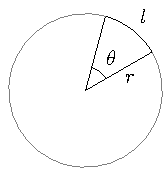
\includegraphics{figAntennaAngleDefinitionRadians}
\caption*{الف: ریڈیئن کی تعریف}
\end{subfigure}%
%
\begin{subfigure}{0.4\textwidth}
\centering
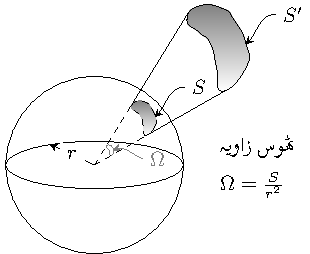
\includegraphics{figAntennaAngleDefinitionSteradians}
\caption*{ب: سٹریڈیئن کی تعریف}
\end{subfigure}%
\caption{ریڈیئن اور سٹریڈیئن کی تعریف}
\label{شکل_اینٹینا_ریڈیئن_تعریف}
\end{figure}

شکل \حوالہ{شکل_اینٹینا_ریڈیئن_تعریف}-ب میں عمومی رقبہ \عددیء{S'} کا محدد کے مرکز پر ٹھوس زاویہ حاصل کرنے کا طریقہ دکھایا گیا ہے۔مرکز سے دیکھتے ہوئے \عددیء{S'} کا بیرونی خاکہ نظر آئے گا۔اگر اس خاکے کے بیرونی کناروں سے  مرکز تک ربڑی چادر کھینچ کر لگائی جائے تو یہ چادر رداس \عددیء{r} کے کرہ کو کاٹے گی۔کرہ کی سطح پر یوں رقبہ \عددیء{S} گھیرا جائے گا۔ٹھوس زاویے
\begin{align}
\Omega=\frac{S}{r^2}
\end{align}
کے برابر ہو گا۔اکائی رداس کے کرہ کی صورت میں رقبہ \عددیء{S} کی قیمت ٹھوس زاویے کی قیمت کے برابر ہو گی۔

شکل \حوالہ{شکل_اینٹینا_ریڈیئن_تعریف}-الف میں \عددیء{\theta}  نظارے کے حدود کو ظاہر کرتا ہے۔اسی طرح شکل \حوالہ{شکل_اینٹینا_ریڈیئن_تعریف}-ب میں \عددیء{\Omega} نظارے  کے حدود تعین کرتا ہے۔

شکل \حوالہ{شکل_اینٹینا_ریڈیئن_تعریف}-الف  میں دکھایا گیا زاویہ سطحی نوعیت کا ہے جسے ریڈیئن میں ناپا جاتا ہے۔اس کے برعکس شکل \حوالہ{شکل_اینٹینا_ریڈیئن_تعریف}-ب  میں دکھایا گیا زاویہ حجمی نوعیت کا ہے جسے سٹریڈیئن یا ریڈیئن کے مربع میں ناپا جاتا ہے۔یاد رہے کہ ایک مربع ریڈیئن کو ہی ایک سٹریڈیئن کہتے ہیں۔
\begin{align}
\SI{1}{\steradian}=\SI{1}{\radian \squared}
\end{align} 

کروی محدد میں \عددیء{r} رداس کے کرہ کی سطح پر رقبے کو
\begin{align}
S=\int_\theta \int_\phi r^2 \sin \theta \dif \theta \dif \phi
\end{align}
لکھا جا سکتا ہے۔یہ رقبہ کرہ کے مرکز پر
\begin{align}
\Omega = \frac{S}{r^2}=\int_\theta \int_\phi \sin \theta \dif \theta \dif \phi \quad \quad (\si{\steradian})
\end{align}
ٹھوس زاویہ بنائے گی۔

\حصہ{موثر رقبہ، سمتیت اور افزائش}
مختصر جفت قطب کے دور میدان میں صرف \عددیء{E_\theta} اور \عددیء{H_\phi} پائے جاتے ہیں جنہیں مساوات \حوالہ{مساوات_اینٹینا_جفت_قطب_دور_میدان} میں پیش کیا گیا ہے۔کسی بھی اینٹینا کی طرح اس کے دور میدان \عددیء{\tfrac{1}{r}} کی شرح سے گھٹتے ہیں لہٰذا پوئنٹنگ  سمتیہ
\begin{align}
\pmb{\mathscr{P}}=\frac{1}{2}\left[\kvec{E}_s \times \kvec{H}_s^* \right]_{\text{حقیقی}} =\frac{Z_0}{2} \abs{H}^2 \ar=\frac{1}{2 Z_0}\abs{E}^2 \ar
\end{align} 
\عددیء{\tfrac{1}{r^2}} کی شرح سے گھٹے گی۔یوں پوئنٹنگ  سمتیہ کے رداسی جزو کو \عددیء{r^2} سے ضرب دینے سے \عددیء{P(\theta,\phi)}
\begin{align}
P(\theta,\phi)=r^2 \mathscr{P}=\frac{Z_0}{2} \abs{H}^2 r^2=\frac{1}{2 Z_0}\abs{E}^2 r^2 \quad \quad (\si{\watt / \steradian})
\end{align} 
حاصل ہوتی ہے جس کی قیمت فاصلہ \عددیء{r} بڑھانے سے نہیں گھٹتی۔\عددیء{P(\theta,\phi)} \اصطلاح{اخراجی شدت}\فرہنگ{اخراجی شدت}\فرہنگ{شدت!اخراجی}\حاشیہب{radiation intensity}\فرہنگ{intensity!radiation} کہلاتی ہے۔اخراجی شدت کے بُعد پر غور کریں۔پوئنٹنگ سمتیہ طاقت کی کثافت  یعنی طاقت فی رقبہ دیتی ہے۔مساوات \حوالہ{مساوات_اینٹینا_ٹھوس_زاویہ_تعریف} سے رقبے کو \عددیء{S=\Omega r^2} لکھا جا سکتا ہے۔یوں پوئنٹنگ سمتیہ ضرب مربع رداس کا بُعد طاقت فی ٹھوس زاویہ \عددیء{\si{\watt/\steradian}} بنتی ہے۔ 

اخراجی شدت کو \اصطلاح{تقابل پذیر}\فرہنگ{تقابل پذیر}\حاشیہب{normalized}\فرہنگ{normalized} بنانے کی خاطر \عددیء{P(\theta,\phi)} کو اس کی زیادہ سے زیادہ قیمت \عددیء{P(\theta,\phi)_{\text{بلندتر}}=r^2 \mathscr{P}_{\text{بلندتر}}} سے تقسیم کرتے ہوئے
\begin{align}
P_n(\theta,\phi)=\frac{P(\theta,\phi)}{P(\theta,\phi)_{\text{بلندتر}}} \quad \quad \text{\RL{بے بُعد}}
\end{align}
بے بُعد\فرہنگ{بے بُعد}\حاشیہب{dimensionless} مقدار \عددیء{P_n(\theta,\phi)} حاصل ہوتی ہے جو  اینٹینا کی \اصطلاح{تقابل پذیر نقش طاقت}\فرہنگ{نقش طاقت!تقابل پذیر}\حاشیہب{normalized power pattern}\فرہنگ{power!normalized pattern}  ہے۔

اینٹینا کی کل اخراج
\begin{align}
\int_0^{2\pi}\int_{0}^{\pi} \mathscr{P} r^2 \sin \theta \dif \theta \dif \phi
\end{align}
ہے۔اگر کثافت طاقت \عددیء{\mathscr{P}_{\text{بلندتر}}} ہو تب اتنی اخراج مکمل کرہ کی سطح کے بجائے  کرہ کی سطح پر رقبہ \عددیء{S} سے خارج ہو گی یعنی
\begin{align}
\mathscr{P}_{\text{بلندتر}} S=\int_0^{2\pi}\int_{0}^{\pi} \mathscr{P} r^2 \sin \theta \dif \theta \dif \phi
\end{align}
ہو گا۔اس میں مساوات \حوالہ{مساوات_اینٹینا_ٹھوس_زاویہ_تعریف} کی مدد سے کرہ کی سطح پر رقبے کو ٹھوس زاویے  کی صورت میں لکھتے ہوئے
\begin{align*}
\Omega_A=\int_0^{2\pi}\int_{0}^{\pi} \frac{\mathscr{P} r^2}{\mathscr{P}_{\text{بلندتر}} r^2 } \sin \theta \dif \theta \dif \phi
\end{align*}
یعنی
\begin{align}\label{مساوات_اینٹینا_اخراجی_ٹھوس_زاویہ}
\Omega_A=\int_0^{2\pi}\int_{0}^{\pi} P_n(\theta,\phi) r^2 \sin \theta \dif \theta \dif \phi=\iint \limits_{4\pi} P_n(\theta,\phi) \dif \Omega \quad \quad (\si{\steradian})
\end{align}
حاصل ہوتا ہے۔اس مساوات کے تحت \عددیء{\Omega_A} ٹھوس زاویے پر یکساں زیادہ سے زیادہ طاقت خارج کرتے ہوئے اینٹینا پوری طاقت خارج کر سکتی ہے۔\عددیء{\Omega_A} کو \اصطلاح{اخراجی ٹھوس زاویہ}\فرہنگ{زاویہ!اخراجی ٹھوس}\فرہنگ{اخراجی ٹھوس زاویہ}\حاشیہب{beam solid angle}\فرہنگ{solid angle!beam} کہتے ہیں۔

اخراجی شعاع کے \اصطلاح{مرکزی گوشے}\فرہنگ{گوشہ!مرکزی}\فرہنگ{مرکزی!گوشہ}\حاشیہب{main lobe}\فرہنگ{main lobe}\فرہنگ{lobe} پر تکمل
\begin{align}
\Omega_M=\iint \limits_{\text{\RL{مرکزی گوشہ}}} P_n(\theta,\phi) \dif \Omega \quad \quad (\si{\steradian})
\end{align}
 لیتے ہوئے \اصطلاح{مرکزی ٹھوس زاویہ}\فرہنگ{ٹھوس!مرکزی زاویہ}\حاشیہب{major lobe solid angle}\فرہنگ{solid angle!major lobe} حاصل کیا جا سکتا ہے۔یوں \اصطلاح{صغیر گوشے}\فرہنگ{گوشہ!صغیر}\حاشیہب{minor lobe}\فرہنگ{lobe!minor} کے ٹھوس زاویہ \عددیء{\Omega_m} کو اخراجی ٹھوس زاویے اور مرکزی ٹھوس زاویے کے فرق
\begin{align}
\Omega_m=\Omega_A-\Omega_M
\end{align}
سے حاصل کیا جا سکتا ہے۔\اصطلاح{غیر سمتی}\فرہنگ{اینٹینا!غیر سمتی}\حاشیہب{isotropic}\فرہنگ{isotropic} اینٹینا ہر سمت میں برابر اخراج کرتی ہے لہٰذا ہر سمت میں اس کا \عددیء{P_n(\theta,\phi)=1} اور \عددیء{\Omega_A=4\pi} ہو گا۔

اینٹینا کی دوسری اہم خاصیت اس کی \اصطلاح{سمتیت}\فرہنگ{سمتیت}\فرہنگ{اینٹینا!سمتیت}\حاشیہب{directivity}\فرہنگ{directivity} ہے۔اخراجی اینٹینا کی زیادہ سے زیادہ اخراجی شدت اور اوسط اخراجی شدت کی شرح
\begin{align}
D=\frac{\text{\RL{زیادہ سے زیادہ اخراجی شدت}}}{\text{\RL{اوسط اخراجی شدت}}} = \frac{P(\theta,\phi)_{\text{بلندتر}}}{P(\theta,\phi)_{\text{اوسط}}} \quad \quad \text{\RL{بے بُعد}}
\end{align}
 اس کی \اصطلاح{سمتیت} کہلاتی ہے۔کل اخراج \عددیء{W} کو \عددیء{4\pi} سٹریڈیئن سے تقسیم کرنے سے اوسط اخراجی شدت \عددیء{P(\theta,\phi)_{\text{اوسط}}} حاصل ہوتی ہے جبکہ اخراجی شدت \عددیء{P(\theta,\phi)} کا \عددیء{4\pi} سٹریڈیئن پر تکمل لینے سے اینٹینا کی کل اخراج حاصل ہوتی ہے۔یوں
\begin{align*}
D=\frac{P(\theta,\phi)_{\text{بلندتر}}}{W/4\pi}&=\frac{4\pi P(\theta,\phi)_{\text{بلندتر}}}{\iint \limits_{4\pi} P(\theta,\phi) \dif \Omega}\\
&=\frac{4\pi}{\iint \limits_{4\pi} \frac{P(\theta,\phi)}{P(\theta,\phi)_{\text{بلندتر}}} \dif \Omega}\\
&=\frac{4\pi}{\iint \limits_{4\pi} P_n(\theta,\phi) \dif \Omega}
\end{align*}
لکھی جا سکتی ہے۔مساوات \حوالہ{مساوات_اینٹینا_اخراجی_ٹھوس_زاویہ} کے ساتھ موازنے کے بعد اسے
\begin{align}\label{مساوات_اینٹینا_سمتیت_ٹھوس_زاویہ_تعلق}
D=\frac{4\pi}{\Omega_A} \quad \quad \text{\RL{بے بُعد}}
\end{align}
لکھا جا سکتا ہے۔یوں اینٹینا کی سمتیت سے مراد، کرہ کا ٹھوس زاویہ \عددیء{4\pi} تقسیم اینٹینا کی اخراجی ٹھوس زاویہ \عددیء{\Omega} ہے۔سمتیت اینٹینا کی ایک منفرد خاصیت ہے۔مخصوص ٹھوس زاویے میں طاقت مرکوز کرنے کی صلاحیت کی ناپ سمتیت ہے۔ سمتیت جتنی زیادہ ہو گی اینٹینا اتنی کم ٹھوس زاویے میں طاقت کو مرکوز کر پائے گا۔

%==================
\ابتدا{مثال}
غیر سمتی اینٹینا کی سمتیت حاصل کریں۔

حل: غیر سمتی اینٹینا ہر سمت میں یکساں اخراج کرتی ہے لہٰذا اس کا \عددیء{P_n(\theta,\phi)=1} اور \عددیء{\Omega_A=1} ہوں گے۔ یوں
\begin{align}
D=\frac{4\pi}{\Omega_A}=1
\end{align}
حاصل ہو گا۔کسی بھی اینٹینا کی یہ کم سے کم ممکنہ سمتیت ہے۔
\انتہا{مثال}
%=================

\ابتدا{مثال}
مختصر جفت قطب کی سمتیت حاصل کریں۔

حل: مساوات \حوالہ{مساوات_اینٹینا_جفت_قطب_دور_میدان} استعمال کرتے ہوئے تقابل پذیر نقش طاقت
\begin{align}
P_n(\theta,\phi)=\frac{H^{2}_{\phi}(\theta,\phi)}{H^{2}_{\phi}(\theta,\phi)_{\text{بلندتر}}}  =\sin^2 \theta
\end{align}
لکھی جا سکتی ہے۔مساوات \حوالہ{مساوات_اینٹینا_اخراجی_ٹھوس_زاویہ} سے
\begin{align}
\Omega_A=\int_0^{2\pi} \int_0^{\pi} \sin^2 \theta \dif \theta \dif \phi=\frac{8\pi}{3} 
\end{align}
اور یوں مساوات  \عددیء{مساوات_اینٹینا_سمتیت_ٹھوس_زاویہ_تعلق} سے
\begin{align}
D=\frac{4\pi}{\Omega}=\frac{3}{2}
\end{align}
حاصل ہوتا ہے۔یوں غیر سمتی اینٹینا کی نسبت سے مختصر جفت قطب کی زیادہ سے زیادہ اخراج \عددیء{\tfrac{3}{2}}  گنا زیادہ ہے۔ 
\انتہا{مثال}
%=============

سمتیت کا دارومدار صرف اور صرف دور میدان کی نقش پر ہے۔اس میں اینٹینا کی کارگزاری شامل نہیں ہے۔اس کے برعکس اینٹینا کی کارگزاری،  اینٹینا کی  افزائش طاقت یا \اصطلاح{افزائش}\فرہنگ{افزائش!اینٹینا}\فرہنگ{اینٹینا!افزائش}\حاشیہب{gain}\فرہنگ{gain}\فرہنگ{antenna!gain} پر اثر انداز ہوتی ہے۔اینٹینا کی افزائش سے مراد
\begin{align}
\text{افزائش} = G = \frac{\text{\RL{آزمائشی اینٹینا کی زیادہ سے زیادہ اخراجی شدت}}}{\text{\RL{حوالہ اینٹینا کی زیادہ سے زیادہ اخراجی شدت}}}
\end{align}
ہے جہاں دونوں اینٹینوں کی داخلی طاقت برابر ہے۔کسی بھی اینٹینا کو بطور حوالہ اینٹینا لیا جا سکتا ہے۔اگر ہم  بے ضیاع، غیر سمتی اینٹینا کو حوالہ تصور کریں تب
\begin{align}
G_0 =\frac{P_m'}{P_0}
\end{align}
ہو گا جہاں
\begin{description}
\جزو{$P_m'$} آزمائشی اینٹینا کی زیادہ سے زیادہ اخراجی شدت،
\جزو{$P_0$} بے ضیاع، غیر سمتی اینٹینا کی اخراجی شدت
\end{description}
ہیں۔یاد رہے کہ غیر سمتی اینٹینا ہر سمت میں یکساں اخراج کرتی ہے لہٰذا اس کی زیادہ سے زیادہ شدت اور اوسط اخراجی شدت برابر ہوتے ہیں۔آزمودہ اینٹینا کی اخراجی شدت \عددیء{P_m'} اور  کامل اینٹینا کی اخراجی شدت \عددیء{P_m} کی شرح اینٹینا کی کارگزاری \عددیء{k} دیتی ہے۔یہ وہی \عددیء{k} ہے جسے مساوات \حوالہ{مساوات_اینٹینا_کارگزاری} میں بھی حاصل کیا گیا۔یوں
\begin{align}
G_0 =\frac{k  P_m}{P_0} = k D
\end{align}
حاصل ہوتا ہے۔یہ مساوات کہتی ہے کہ کسی بھی کامل اینٹینا \عددیء{(k=\SI{100}{\percent})} کی افزائش، کامل غیر سمتی اینٹینا کی نسبت سے، اسی اینٹینا کی سمتیت کے برابر ہوتی ہے۔ غیر کامل \عددیء{k < \SI{100}{\percent}} اینٹینا کی صورت میں افزائش کی قیمت سمتیت سے کم ہو گی۔

سمتیت کی قیمت \عددیء{1} تا \عددیء{\infty} ممکن ہے۔سمتیت کی قیمت  اکائی سے کم نہیں ہو سکتی۔اس کے برعکس افزائش کی قیمت صفر تا لا محدود ممکن ہے۔
\begin{align*}
1 \le &D \le \infty\\
0 \le & G \le \infty \quad \quad \text{\RL{ممکنہ قیمت}}
\end{align*}

\begin{figure}
\centering
\begin{subfigure}{0.4\textwidth}
\centering
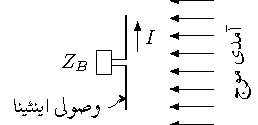
\includegraphics{figAntennaReceivingAntennaToLoad}
\caption*{الف: آمدی موج میں تر وصولی اینٹینا}
\end{subfigure}%
%
\begin{subfigure}{0.4\textwidth}
\centering
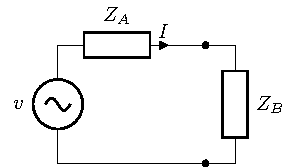
\includegraphics{figAntennaReceivingAntennaToLoadSchematic}
\caption*{ب: اینٹینا کے ساتھ برقی رکاوٹ جوڑا گیا ہے}
\end{subfigure}%
\caption{وصولی اینٹینا آمدی موج سے طاقت حاصل کر کے برقی رکاوٹ کو فراہم کرتی ہے۔}
\label{شکل_اینٹینا_وصولی_اینٹینا_اور_موج}
\end{figure}

\اصطلاح{اخراجی اینٹینا}\فرہنگ{اخراجی!اینٹینا}\فرہنگ{اینٹینا!اخراجی}\حاشیہب{transmitting antenna}\فرہنگ{antenna!transmitting}\فرہنگ{transmitting!antenna} شعاعی اخراج کرتی ہے۔اس کے برعکس \اصطلاح{وصولی اینٹینا}\فرہنگ{وصولی!اینٹینا}\فرہنگ{اینٹینا!وصولی}\حاشیہب{receiving antenna}\فرہنگ{antenna!receiving}\فرہنگ{receiving!antenna} شعاع سے طاقت وصول کرتی ہے۔برقی و مقناطیسی امواج جب وصولی اینٹینا پر پہنچتے ہیں تو وصولی اینٹینا ان سے طاقت حاصل کرتی ہے۔اگر اینٹینا کے برقی سروں پر بیرونی مزاحمت \عددیء{R_B} نسب کی جائے تو حاصل کردہ طاقت کا کچھ حصہ اس مزاحمت میں ضائع ہو گا۔ہم چونکہ بیرونی مزاحمت کو فراہم طاقت \عددیء{W=I^2 R_B} میں دلچسپی رکھتے ہیں لہٰذا اسی کی بات کرتے ہوئے آگے بڑھتے ہیں۔بیرونی مزاحمت کو فراہم طاقت \عددیء{I^2 R_B} کے برابر طاقت آمدی موج کے رقبہ \عددیء{S} میں پایا جاتا ہے۔یوں
\begin{align}
 \mathscr{P} S=I^2 R_B
\end{align} 
لکھا جا سکتا ہے۔ہم فرض کرتے ہیں کہ اینٹینے کا رقبہ \عددیء{S} ہی ہے اور اینٹینا اتنے رقبے پر  آمدی موج سے مکمل طاقت حاصل کرنے اور اسے بیرونی برقی سروں تک منتقل کرنے  کی صلاحیت رکھتی ہے۔اس فرضی رقبے کو \اصطلاح{وصولی رقبہ}\فرہنگ{رقبہ!وصولی}\فرہنگ{اینٹینا!وصولی رقبہ}\حاشیہب{antenna aperture}\فرہنگ{antenna!aperture}\فرہنگ{aperture} کہا جاتا ہے۔یوں وصولی رقبے کو
\begin{align}
S=\frac{I^2 R_B}{\mathscr{P}}
\end{align}
سے حاصل کیا جا سکتا ہے جہاں
\begin{description}
\جزو{$A$} اینٹینا کا فرضی رقبہ، $\si{\meter \squared}$
\جزو{$I$} موثر برقی رو، $\si{\ampere}$
\جزو{$\mathscr{P}$} آمدی موج کا پوئنٹنگ سمتیہ، $\si{\watt /\meter \squared}$
\جزو{$R_L$} برقی مزاحمت، $\si{\ohm}$
\end{description}
ہیں۔حقیقت میں اینٹینا \عددیء{I^2 R_B} سے زیادہ طاقت حاصل کرتی ہے جس کا کچھ حصہ اینٹینا کے اندر ہی ضائع ہو جاتا ہے۔ہمیں اینٹینا کے اندر ضائع ہونے والے طاقت سے کوئی دلچسپی نہیں ہے۔

شکل \حوالہ{شکل_اینٹینا_وصولی_اینٹینا_اور_موج}-الف میں آمدی موج میں تر اینٹینا دکھایا گیا ہے جسے بیرونی برقی رکاوٹ \عددیء{Z_B} کے ساتھ جوڑا گیا ہے۔اینٹینا کا \اصطلاح{تھونن}\فرہنگ{تھونن}\حاشیہب{Thevenin equivalent circuit}\فرہنگ{Thevenin} مساوی دور استعمال کرتے ہوئے،  شکل-ب میں اسی کا  مکمل برقی دور دکھایا گیا ہے۔اس دور میں سلسلہ وار برقی رو
\begin{align*}
I=\frac{v}{Z_A+Z_B}=\frac{v}{R_A+R_B+j(X_A+X_B)}
\end{align*}
ہو گی جہاں
\begin{description}
\جزو{$v$} اینٹینا میں آمدی موج سے پیدا موثر برقی دباو،
\جزو{$R_A$} اینٹینا کے تھونن مساوی دور میں اینٹینا کی مزاحمت،
\جزو{$X_A$} تھونن دور میں اینٹینا کی متعاملیت،
\جزو{$R_B$} بیرونی مزاحمت،
\جزو{$X_B$} بیرونی متعاملیت
\end{description}
ہیں۔یوں بیرونی مزاحمت کو مہیا طاقت 
\begin{align}
\abs{I}^2 R_B=\frac{v^2 R_B}{(R_A+R_B)^2+(X_A+X_B)^2}
\end{align}
ہو گا جس سے  اینٹینے کا رقبہ وصولی
\begin{align}
S=\frac{v^2 R_B}{\mathscr{P}\left[(R_A+R_B)^2+(X_A+X_B)^2\right]}
\end{align}
حاصل ہوتا ہے۔ 

آمدی موج کی نسبت سے ایک مخصوص انداز میں رکھے ہوئے اینٹینا میں زیادہ سے زیادہ برقی دباو پیدا ہو گا۔اسی جگہ اینٹینا کو رکھتے ہوئے بیرونی مزاحمت میں زیادہ سے زیادہ طاقت اس صورت منتقل ہو گی جب
\begin{align}
R_B&=R_A\\
X_B&=-X_A
\end{align}
ہوں۔بے ضیاع اینٹینا کی تھونن مزاحمت دراصل اینٹینا کی اخراجی مزاحمت \عددیء{R_r} ہی ہے۔اس طرح بیرونی مزاحمت میں زیادہ سے زیادہ طاقت منتقل کرتے وقت زیادہ سے زیادہ وصولی رقبہ
\begin{align}\label{مساوات_اینٹینا_موثر_رقبہ_اینٹینا}
S_{\text{موثر}} = \frac{v^2}{4\mathscr{P} R_r }
\end{align}
 حاصل ہو گا جسے اینٹینا کا \اصطلاح{موثر رقبہ}\فرہنگ{اینٹینا!موثر رقبہ}\فرہنگ{موثر!رقبہ اینٹینا}\حاشیہب{effective aperture}\فرہنگ{effective!aperture} \عددیء{S_{\text{موثر}}} پکارا جاتا ہے۔ہر اینٹینا مخصوص قیمت کا \اصطلاح{موثر رقبہ} رکھتا ہے۔

%=========================
\ابتدا{مثال}
پورے مختصر جفت قطب پر یکساں برقی رو تصور کرتے ہوئے، اس کا موثر رقبہ حاصل کریں۔

حل:مساوات \حوالہ{مساوات_اینٹینا_موثر_رقبہ_اینٹینا} سے ظاہر ہے کہ موثر رقبہ دریافت کرنے کے لئے، اینٹینا میں پیدا برقی دباو \عددیء{v}، اینٹینا کی اخراجی مزاحمت \عددیء{R_r} اور آمدی موج میں کثافت طاقت \عددیء{\mathscr{P}} درکار ہوں گے۔جفت قطب میں زیادہ سے زیادہ برقی دباو اس صورت پیدا ہو گی جب اینٹینا کی تار اور آمدی موج کا برقی میدان متوازی ہوں۔ایسی صورت میں اینٹینا میں
\begin{align}
v=E l
\end{align}
برقی دباو پیدا ہو گی۔آمدی موج کی پوئنٹنگ سمتیہ
\begin{align}
\mathscr{P}=\frac{E^2}{Z_0} \quad \quad (\si{\watt/ \meter \squared})
\end{align}
ہے جہاں \عددیء{Z_0=\sqrt{\mu_0/\epsilon_0}=120 \pi} خالی خلاء کی قدرتی رکاوٹ ہے۔مساوات \حوالہ{مساوات_اینٹینا_اخراجی_مزاحمت_جفت_قطب} میں \عددیء{I=I_0} پر کرنے سے موجودہ جفت قطب کی اخراجی مزاحمت
\begin{align}
R_r=80 \pi^2 \left(\frac{l}{\lambda}\right)^2
\end{align}
حاصل ہوتی ہے۔ان تمام کو مساوات \حوالہ{مساوات_اینٹینا_موثر_رقبہ_اینٹینا} میں پر کرتے ہوئے
\begin{align}
S_{\text{موثر}} = \frac{E^2 l^2}{4 \frac{E^2}{Z_0} 80 \pi^2 \left(\frac{l}{\lambda}\right)^2  }=\frac{3\lambda^2}{8\pi}=0.119 \lambda^2 \quad \quad (\si{\meter \squared})
\end{align}
\انتہا{مثال}
%=======================

یوں کامل مختصر جفت قطب کی لمبائی جتنی بھی کم کیوں نہ ہو یہ ہر صورت \عددیء{0.119 \lambda^2} موثر رقبے پر آمدی موج سے تمام طاقت حاصل کرنے اور اسے بیرونی مزاحمت تک منتقل کرنے کی صلاحیت رکھتا ہے۔حقیقی جفت قطب غیر کامل ہو گا  لہٰذا اس کی مزاحمت \عددیء{R_{\text{اخراجی}}+R_{\text{ضائع}}} ہو گی۔یوں کامل جفت قطب کا موثر رقبہ کچھ کم ہو گا۔

آئیں ایسے اینٹینا کی بات کریں جس کا موثر رقبہ \عددیء{S_{\text{موثر}}} اور اخراجی ٹھوس زاویہ \عددیء{\Omega_A} ہو۔موثر رقبے پر یکساں برقی میدان \عددیء{E_m} کی صورت میں اخراجی طاقت
\begin{align}
P=\frac{E_m^2}{Z} S_{\text{موثر}}
\end{align}
ہو گا جہاں \عددیء{Z} انتقالی خطے کی قدرتی رکاوٹ ہے۔

اگر \عددیء{r} فاصلے پر میدان \عددیء{E_r} ہو تب اخراجی طاقت
\begin{align}
P=\frac{E_r^2}{Z} r^2 \Omega_A
\end{align}
ہو گا۔ 

ہم آگے جا کر ایک نتیجہ حاصل کریں گے جس کے تحت  \عددیء{E_r=\tfrac{E_m A_{\text{موثر}}}{r \lambda}} ہے۔اس نتیجے کو استعمال کرتے ہوئے مندرجہ بالا دو مساوات کو برابر لکھتے ہوئے
\begin{align}\label{مساوات_اینٹینا_اخراجی_ٹھوس_زاویہ_موثر_رقبہ_تعلق}
\lambda^2 =A_{\text{موثر}} \Omega_A \quad \quad (\si{\meter \squared})
\end{align}
حاصل ہوتا ہے جہاں
\begin{description}
\جزو{$\lambda$} طول موج،
\جزو{$A_{\text{موثر}}$}  اینٹینا کا موثر رقبہ اور
\جزو{$\Omega_A$} اینٹینا کا اخراجی ٹھوس زاویہ
\end{description}
ہیں۔اس مساوات کے تحت اینٹینا کا موثر رقبہ ضرب اخراجی ٹھوس زاویہ برابر ہوتا ہے  طول موج کا مربع۔یوں اگر ہمیں موثر رقبہ معلوم ہو تب ہم اخراجی ٹھوس زاویہ حاصل کر سکتے ہیں اور اگر اخراجی ٹھوس زاویہ معلوم ہو تب موثر رقبہ حاصل کیا جا سکتا ہے۔

مساوات \حوالہ{مساوات_اینٹینا_سمتیت_ٹھوس_زاویہ_تعلق} میں مساوات \حوالہ{مساوات_اینٹینا_اخراجی_ٹھوس_زاویہ_موثر_رقبہ_تعلق} پر کرنے سے
\begin{align}
D=\frac{4\pi}{\lambda^2} A_{\text{موثر}}
\end{align}
لکھا جا سکتا ہے۔سمتیت کی یہ تیسری مساوات ہے۔تینوں کو یہاں دوبارہ پیش کرتے ہیں

\begin{gather}
\begin{aligned}
D&=\frac{P(\theta,\phi)_{\text{بلندتر}}}{P_{\text{اوسط}}} \\
D&=\frac{4\pi}{\Omega} \\
D&=\frac{4\pi}{\lambda^2} A_{\text{موثر}}
\end{aligned}
\end{gather}
جہاں پہلی دو مساوات میں سمتیت اخراجی شعاع کے نقش سے حاصل کی گئی ہے جبکہ تیسری مساوات میں اسے موثر رقبے سے حاصل کیا گیا ہے۔

\حصہ{قطاری ترتیب}
مسئلہ اینٹینا دراصل اینٹینا کے مختلف حصوں سے پیدا میدانوں کا درست مجموعہ حاصل کرنا ہے۔اینٹینا کے مختلف حصوں کے میدان جمع کرتے ہوئے ان کے انفرادی حیطے اور زاویائی فرق کا خیال رکھنا ضروری ہے۔

\جزوحصہ{غیر سمتی، دو نقطہ منبع}
 دو عدد نقطہ منبع کو شکل میں دکھایا گیا ہے۔دونوں منبع غیر سمتی ہیں اور ان کے درمیان فاصلہ \عددیء{d} ہے۔نقطہ منبع سے مراد ایسی فرضی منبع ہے جس کا حجم صفر کے برابر ہو۔ ہم آگے چل کر \اصطلاح{مسئلہ متکافیت}\فرہنگ{مسئلہ!متکافیت}\فرہنگ{اینٹینا!متکافیت}\حاشیہب{reciprocity}\فرہنگ{reciprocity} دیکھیں گے جس کے تحت نقطہ منبع کے قطاروں کا اخراجی نقش اور انہیں کا وصولی نقش بالکل یکساں ہوتے ہیں۔    

ہم فرض کرتے ہیں کہ دونوں منبع برابر حیطے اور ہم قدم میدان پیدا کرتے ہیں۔دونوں میدان کے خطی تقطیب ہیں۔مزید یہ کہ دونوں کے \عددیء{\kvec{E}} میدان صفحے کے عمودی ہیں۔دونوں منبع سے برابر فاصلے پر ان کے بالکل درمیانے مقام پر زاویائی صفر تصور کرتے ہوئے، دور میدان کو
\begin{align}
E=E_2 e^{j\frac{\psi}{2}} + E_1 e^{-j \frac{\psi}{2}}
\end{align}
لکھا جا سکتا ہے جہاں
\begin{align}
\psi=\beta d \cos \theta=\frac{2\pi d}{\lambda}\cos \theta
\end{align}
ہے۔ان مساوات میں 
\begin{description}
\جزو{$E_1$} منبع-1 کا زاویہ \عددیء{\theta} سمت میں دور میدان،
\جزو{$E_2$} منبع-2 کا زاویہ \عددیء{\theta} سمت میں دور میدان اور
\جزو{$\psi$} دونوں اشارات کا زاویہ \عددیء{\theta} کی سمت میں زاویائی فرق
\end{description}
ہیں۔دونوں دور میدان برابر \عددیء{(E_1=E_2)} ہونے کی صورت میں یوں
\begin{align}\label{مساوات_اینٹینا_دو_نقطہ_الف}
E=E_1 \left(e^{j\frac{\psi}{2}} + e^{-j \frac{\psi}{2}} \right)=2 E_1 \cos \frac{\psi}{2}
\end{align}
ہو گا۔ فاصلہ \عددیء{d=\frac{\lambda}{2}}  کی صورت میں میدان کو شکل میں دکھایا گیا ہے۔

اگر زاویائی صفر کو دونوں منبع کے درمیانے مقام کی جگہ منبع-1 پر چنا جاتا تب دور میدان
\begin{gather}
\begin{aligned}
E&=E_1+E_2 e^{j \psi}\\
&=\left(E_1 e^{-j\frac{\psi}{2}}+E_2 e^{j \frac{\psi}{2}}\right) e^{j\frac{\psi}{2}}
\end{aligned}
\end{gather}
حاصل ہوتا جو \عددیء{E_1=E_2} کی صورت میں 
\begin{align}\label{مساوات_اینٹینا_دو_نقطہ_ب}
E=2 E_1 \cos \frac{\psi}{2} e^{j\frac{\psi}{2}}=2 E_1 \cos \frac{\psi}{2} \phase{\tfrac{\psi}{2}}
\end{align}
حاصل ہوتا۔میدان کا نقش  چونکہ میدان کے حیطے پر منحصر ہوتا ہے لہٰذا اس میں کوئی تبدیلی رونما نہیں ہوئی البتہ میدان کا زاویہ تبدیل ہو گیا ہے۔میدان کے زاویے کی تبدیلی کی وجہ یہ ہے کہ ہم نے زاویے کے صفر کو دونوں منبع کے درمیانے مقام سے ہٹا کر منبع-1 پر چنا ہے۔

\جزوحصہ{ضرب نقش}
گزشتہ حصے میں بالکل یکساں دو عدد غیر سمتی نقطہ منبع کے میدان پر غور کیا گیا۔اگر نقطہ منبع سمتی ہوں  اور دونوں کے نقش بالکل یکساں ہوں تب بھی مساوات \حوالہ{مساوات_اینٹینا_دو_نقطہ_الف} (یا مساوات \حوالہ{مساوات_اینٹینا_دو_نقطہ_ب}) ہی ان کا مجموعی میدان دے گا پس فرق اتنا ہے کہ اب \عددیء{E_1} از خود \عددیء{\theta} کا تفاعل \عددیء{E(\theta)} ہے۔ انفرادی نقطہ منبع کے نقش \عددیء{E_1(\theta)} کو \اصطلاح{ابتدائی نقش}\فرہنگ{ابتدائی!نقش}\فرہنگ{نقش!ابتدائی}\حاشیہب{primary pattern}\فرہنگ{pattern!primary} جبکہ \عددیء{\cos \tfrac{\psi}{2}} کو \اصطلاح{ثانوی نقش}\فرہنگ{ثانوی!نقش}\فرہنگ{نقش!ثانوی}\حاشیہب{secondary pattern}\فرہنگ{pattern!secondary} یا \اصطلاح{قطاری نقش}\فرہنگ{قطار! قطاری نقش}\فرہنگ{نقش!قطاری}\حاشیہب{array pattern}\فرہنگ{pattern!array}\فرہنگ{array!pattern} کہا جائے گا۔یوں
\begin{align}\label{مساوات_اینٹینا_ضرب_نقش}
E=E(\theta) \cos \frac{\psi}{2}
\end{align}
لکھا جا سکتا ہے۔مساوات \حوالہ{مساوات_اینٹینا_ضرب_نقش} \اصطلاح{ضرب نقش}\فرہنگ{نقش!ضرب}\فرہنگ{ضرب نقش}\حاشیہب{pattern multiplication}\فرہنگ{pattern!multiplication} کا اصول بیان کرتا ہے جس کے تحت انفرادی منبع کا نقش اور غیر سمتی نقطہ منبع کے قطار کا نقش ضرب دینے سے سمتی منبع کے قطار کا نقش حاصل ہوتا ہے۔یہاں فرض کیا گیا ہے کہ قطار میں انفرادی نقطہ منبع کا نقش وہی ہے جو اس نقطہ منبع کا تنہائی میں نقش ہوتا ہے۔

\جزوحصہ{ثنائی قطار}
مساوات \حوالہ{مساوات_اینٹینا_دو_نقطہ_ب} دو غیر سمتی زاویائی طور پر ہم قدم نقطہ منبع کے جوڑی کا دور میدان دیتا ہے۔نقطہ منبع کے درمیان فاصلہ \عددیء{\tfrac{\lambda}{2}} اور \عددیء{E_1=\tfrac{1}{2}} ہونے کی صورت میں اس مساوات کو
\begin{align}
E=\cos \left(\frac{\pi}{2}\cos \theta\right)
\end{align}
لکھا جا سکتا ہے۔یہاں \عددیء{E_1=\tfrac{1}{2}}  چنے سے نقش پر توجہ رکھنا نسبتاً آسان ہو جاتا ہے۔اس نقش کو شکل میں دکھایا گیا ہے جس میں کوئی صغیر گوشہ نہیں پایا جاتا۔ اس جوڑی منبع کے سیدھ میں \عددیء{\tfrac{\lambda}{2}} فاصلے پر منبع کی دوسری جوڑی رکھنے سے شکل-ب حاصل ہوتا ہے۔اس شکل میں دو درمیانے منبع دراصل ایک ہی نقطے پر پائے جائیں گے لیکن وضاحت کی خاطر انہیں اوپر نیچے دکھایا گیا ہے۔ضرب نقش کے اصول کے تحت ان کا مجموعی میدان
\begin{align}
E=\cos^2 \left(\frac{\pi}{2}\cos \theta\right)
\end{align}
ہو گا جسے شکل میں دکھایا گیا ہے۔اس قطار کو تین عدد منبع کی قطار تصور کیا جا سکتا ہے جہاں قطار میں بالترتیب، منبع کی طاقت \عددیء{(1:2:1)} نسبت سے ہے۔اس تین رکنی قطار کے سیدھ میں لیکن \عددیء{\tfrac{\lambda}{2}} ہٹ کر بالکل ایسی ہی تین رکنی قطار رکھنے سے شکل حاصل ہوتی ہے۔اس نئی قطار کو چار رکنی تصور کیا جا سکتا ہے جہاں بالترتیب منبع کی طاقت \عددیء{(1:3:3:1)} نسبت سے ہے۔ اس چار رکنی قطار کا میدان
\begin{align}
E=\cos^3 \left(\frac{\pi}{2}\cos \theta\right)
\end{align}
ہے۔اس نقش میں بھی صغیر گوشہ نہیں پایا جاتا۔اسی طرح بڑھتے ہوئے، صغیر گوشے سے پاک، زیادہ سے زیادہ سمتیت کا نقش حاصل کیا جا سکتا ہے۔یوں زیادہ منبع پر مبنی قطار میں منبع کی طاقت \اصطلاح{ثنائی تسلسل}\فرہنگ{ثنائی!تسلسل}\فرہنگ{تسلسل!ثنائی}\حاشیہب{binomial series}\فرہنگ{binomial series} کے \اصطلاح{ثنائی سر}\حاشیہب{binomial coefficient} کی نسبت سے ہوتے ہیں۔ ثنائی سروں کو شکل میں دکھائے گئے \اصطلاح{پاسکل تکون}\فرہنگ{پاسکل تکون}\فرہنگ{تکون!پاسکل}\حاشیہب{Pascal triangle}\فرہنگ{Pascal triangle} کی مدد سے حاصل کیا جا سکتا ہے جس میں ہر اندرونی عدد، اوپر کے قریبی دو اعداد کا مجموعہ ہوتا ہے۔متعدد منبع کے قطار کا نقش
\begin{align}
E=\cos^{n-1} \left(\frac{\pi}{2}\cos \theta\right)
\end{align}
کے برابر ہو گا جہاں قطار میں منبع کی تعداد \عددیء{n} ہے۔

اگرچہ مندرجہ بالا \عددیء{n} رکنی  قطار کے نقش میں کوئی صغیر گوشہ نہیں پایا جاتا اس کے باوجود اس کی سمتیت برابر طاقت کے \عددیء{n} رکنی منبع کے قطار سے کم ہوتی ہے۔حقیقی قطار عموماً ان دو صورتوں (ثنائی قطار اور یکساں قطار) کی درمیانی شکل رکھتے ہیں۔  
